\documentclass[12pt,a4paper]{article}
\usepackage[utf8]{inputenc}
\usepackage[T1]{fontenc}
\usepackage{amsmath}
\usepackage{amssymb}
\usepackage{graphicx}
\usepackage{xcolor}
\usepackage[a4paper, margin=2.5cm]{geometry}
\usepackage{hyperref}
\usepackage{xurl}
\usepackage{tabularx}
\usepackage{float}
\usepackage{booktabs}
\usepackage{longtable}
\usepackage{array}
\usepackage{enumitem}
\usepackage{fancyhdr}
\usepackage{titlesec}
\usepackage{listings}
\usepackage{caption}
\captionsetup{font=small,labelfont=bf}

% ---------- Colores institucionales ----------
\definecolor{utedark}{HTML}{1B3A5C}
\definecolor{uteprimary}{HTML}{2E86AB}
\definecolor{uteaccent}{HTML}{A23B72}
\definecolor{utelight}{HTML}{F0F3F5}
\definecolor{codebg}{HTML}{F5F5F5}

\hypersetup{colorlinks=true,linkcolor=utedark,urlcolor=uteprimary}

% ---------- Portada ----------
\title{\vspace{2.5cm}
{\Huge\textcolor{utedark}{Evaluación de la Unidad 2}}\\[0.4cm]
{\LARGE Extracción de Conocimiento de Base de Datos}\\[1.2cm]
{\large Análisis Supervisado y No Supervisado (SA, NS, DE) y Herramienta Alternativa (AU)}}
\author{}
\date{}

\setlength{\parindent}{0pt}
\setlength{\parskip}{6pt}
\renewcommand{\contentsname}{Índice}
\renewcommand{\refname}{Referencias}
\renewcommand{\tablename}{Tabla}

\titleformat{\section}{\Large\bfseries\color{utedark}}{\thesection.}{0.6em}{}
\titleformat{\subsection}{\large\bfseries\color{uteprimary}}{\thesubsection.}{0.6em}{}
\titleformat{\subsubsection}{\normalsize\bfseries\color{uteaccent}}{\thesubsubsection.}{0.6em}{}

\pagestyle{fancy}
\fancyhf{}
\fancyhead[L]{\small\textcolor{utedark}{Extracción de Conocimiento de Base de Datos}}
\fancyhead[R]{\small\textcolor{utedark}{Evaluación Unidad 2}}
\renewcommand{\headrulewidth}{0.4pt}
\renewcommand{\headrule}{\hbox to\headwidth{\color{uteprimary}\leaders\hrule height \headrulewidth\hfill}}
\fancyfoot[C]{\thepage}

\lstset{basicstyle=\ttfamily\small,backgroundcolor=\color{codebg},frame=single,
        rulecolor=\color{gray!60},breaklines=true}

\begin{document}

% ================= PORTADA =================
\thispagestyle{empty}
\begin{center}
\vspace*{0.3cm}

\vspace{0.6cm}
{\Large Universidad Tecnológica de Querétaro}\\[0.2cm]
{\large División de Automatización e Información}\\[0.2cm]
{\large Ingeniería en Gestión de Desarrollo de Software}

\vspace{1.2cm}
{\Huge\bfseries\textcolor{utedark}{Evaluación de la Unidad 2}}\\[0.5cm]
{\LARGE\bfseries Extracción de Conocimiento de Base de Datos}\\[1.0cm]
{\large Análisis Supervisado y No Supervisado}\\[0.3cm]
{\large Reporte de algoritmos de regresión, clasificación, agrupación, reducción de dimensionalidad y herramienta alternativa}

\vspace{1.2cm}
\begin{tabular}{rl}
\textbf{Materia:} & Extracción de Conocimiento de Base de Datos \\
\textbf{Docente:} & Filiberto Ruíz Hernández \\
\textbf{Semestre:} & 2026 \\
\textbf{Alumno:} & Ramírez Martínez Mario Alberto \\
\textbf{Matrícula:} & 2023371044 \\
\textbf{Fecha:} & 2026-08-07 \\
\end{tabular}

\vspace{1.0cm}
{\large\textbf{Datasets:} beisbol.csv, breast-cancer.csv, samsung.csv, comprar\_alquilar.csv}

\end{center}
\newpage

% ================= ÍNDICE =================
{\hypersetup{linkcolor=utedark}\tableofcontents}
\newpage

% ================= 1. INTRODUCCIÓN =================
\section{Introducción}

\subsection{Objetivo}
La presente evaluación de la Unidad 2 tiene como objetivo aplicar técnicas de
\textbf{aprendizaje supervisado} (regresión y clasificación) y \textbf{aprendizaje no
supervisado} (agrupación y reducción de dimensionalidad) sobre cuatro conjuntos de
datos, así como implementar una \textbf{herramienta alternativa} a Jupyter Notebook
para resolver los ejercicios de las evaluaciones SA y DE.

\subsection{Conjuntos de datos}
\begin{longtable}{@{}>{\raggedright\arraybackslash}p{4.6cm}>{\raggedright\arraybackslash}p{7.2cm}>{\raggedright\arraybackslash}p{3.2cm}@{}}
\caption{Conjuntos de datos de la evaluación}\\
\toprule
\textbf{Archivo} & \textbf{Descripción} & \textbf{Problema} \\
\midrule
\endfirsthead
\toprule
\textbf{Archivo} & \textbf{Descripción} & \textbf{Problema} \\
\midrule
\endhead
\texttt{beisbol.csv} & 30 equipos de béisbol: \texttt{bateos} y \texttt{runs} & Regresión \\
\texttt{breast-cancer.csv} & 569 casos de cáncer de mama, 30 características y diagnóstico (B/M) & Clasificación \\
\texttt{samsung.csv} & 2,850 días de cotización de la acción Samsung (Close y Volume) & Agrupación \\
\texttt{comprar\_alquilar.csv} & 202 registros con 9 variables financieras y decisión comprar/alquilar & Reducción de dimensionalidad \\
\bottomrule
\end{longtable}

\subsection{Repositorio}
Todos los notebooks, modelos y reportes se encuentran en el repositorio:
\begin{center}
\url{https://github.com/rmMarioAlberto/evaluacion-u2-extraccion-conocimiento-bd}
\end{center}
Cada sección de este documento incluye el enlace al modelo obtenido en dicho
repositorio (carpeta \texttt{modelos/} y notebook correspondiente en \texttt{notebooks/}).

% ================= 2. SA REGRESIÓN =================
\section{Análisis Supervisado 1 — Regresión sobre beisbol.csv}

\subsection{Justificación del algoritmo}
Se eligió \textbf{Regresión Lineal Simple} porque la variable objetivo
\texttt{runs} es continua y existe un único predictor numérico (\texttt{bateos}).
Es el modelo más simple e interpretable: la pendiente indica cuántas carreras
adicionales produce cada turno al bat extra. Con solo 30 observaciones, un modelo
más complejo (árboles, redes) se sobreajustaría con facilidad, por lo que la
regresión lineal ofrece una línea de base robusta y auditable.

\subsection{Diseño del modelo (paso a paso)}
\begin{enumerate}[itemsep=2pt]
\item \textbf{Carga y exploración:} se lee \texttt{beisbol.csv}; no hay valores nulos.
\item \textbf{Análisis exploratorio:} el diagrama de dispersión muestra una tendencia
      creciente; la correlación entre \texttt{bateos} y \texttt{runs} es
      $r = 0.6106$.
\item \textbf{Estrategia de evaluación:} al haber solo 30 observaciones, reservar un
      conjunto de prueba de 6--9 filas hace el $R^2$ de prueba inestable. Por ello se
      evalúa con \textbf{validación cruzada} usando \textbf{RMSE} (métrica bien
      definida incluso con pliegues de una muestra): \texttt{LeaveOneOut} (LOOCV) y
      k-fold (5 pliegues).
\item \textbf{Entrenamiento:} se ajusta el modelo lineal sobre los 30 equipos.
\item \textbf{Optimización:} búsqueda de hiperparámetros mediante
      \texttt{GridSearchCV} sobre el grado de una regresión polinomial (1--4).
\end{enumerate}

\subsection{Evaluación y optimización}
\begin{table}[H]
\centering
\caption{Métricas del modelo de regresión lineal (beisbol.csv)}
\begin{tabular}{lcc}
\toprule
\textbf{Métrica} & \textbf{Ajuste completo} & \textbf{Validación cruzada} \\
\midrule
$R^2$ & 0.3729 & --- \\
RMSE & 64.22 & LOOCV: 55.59 \;/\; 5-fold: 69.23 \\
MAE & 51.67 & --- \\
\bottomrule
\end{tabular}
\end{table}

La ecuación ajustada es:
\[
\widehat{\text{runs}} = 0.6305 \times \text{bateos} - 2789.2429
\]

\textbf{Búsqueda de hiperparámetros (grado polinomial).} El \texttt{GridSearchCV}
evaluó grados 1 a 4:
\begin{table}[H]
\centering
\caption{Comparación de grados polinomiales (RMSE de validación cruzada)}
\begin{tabular}{cc}
\toprule
\textbf{Grado} & \textbf{RMSE (CV)} \\
\midrule
1 & 69.230 \\
2 & 69.078 \\
3 & 68.926 \\
4 & 69.233 \\
\bottomrule
\end{tabular}
\end{table}

Los grados superiores reducen el RMSE en menos de 0.4 carreras (aproximadamente
0.5\%), una mejora marginal que no justifica la complejidad añadida ni el riesgo de
sobreajuste. Por parsimonia (principio de Occam) se conserva la regresión lineal
simple (grado 1) como modelo final.

\subsection{Gráficas e interpretación de resultados}
\begin{figure}[H]
\centering
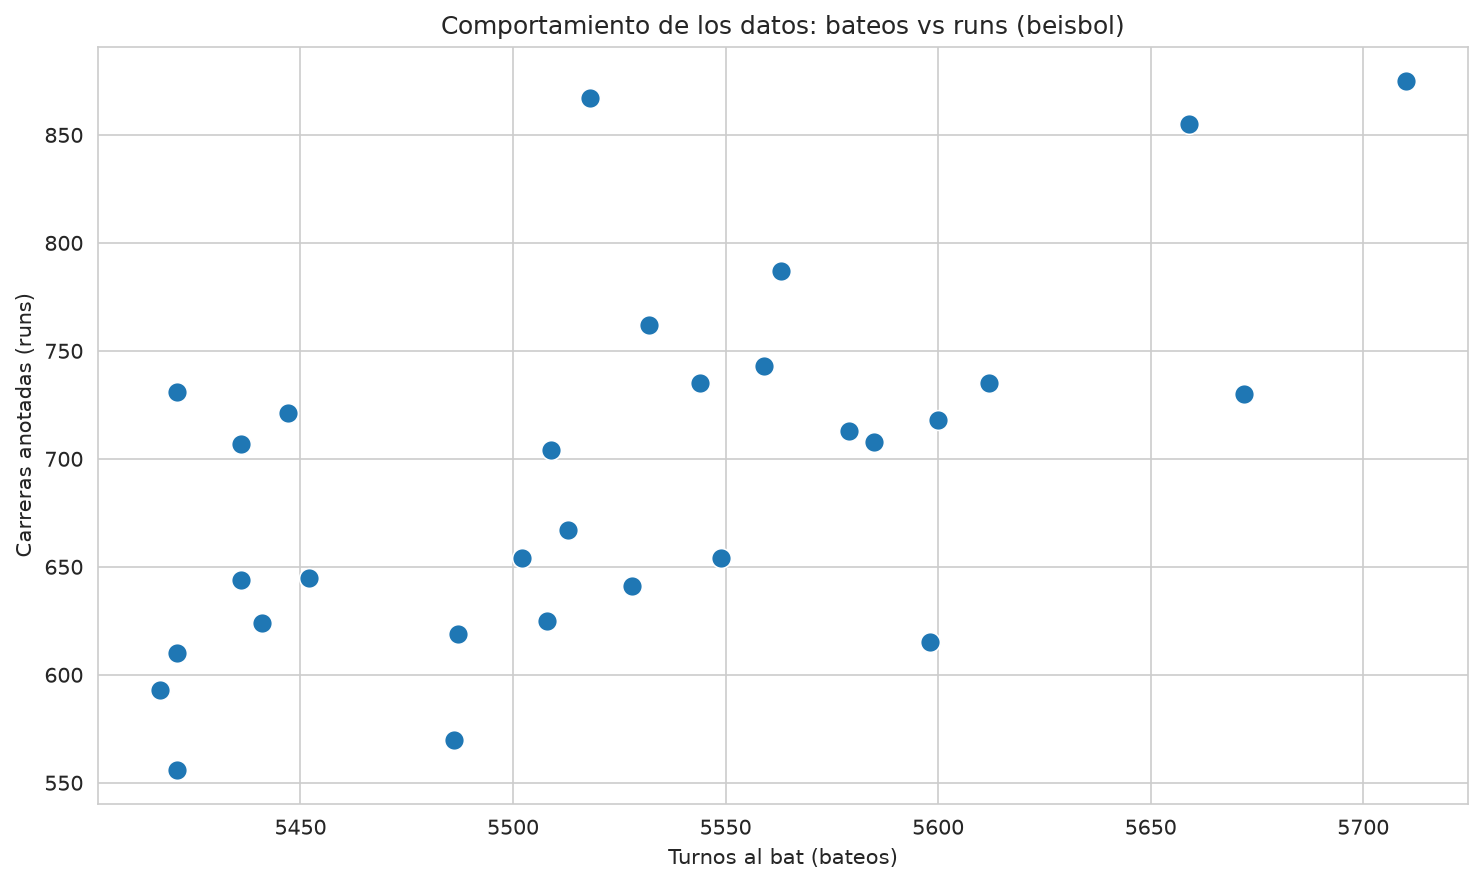
\includegraphics[width=0.82\linewidth]{img/scatter_beisbol.png}
\caption{Dispersión del comportamiento de los datos: bateos vs runs. Se observa una
tendencia lineal creciente moderada ($r=0.61$), con varios equipos por encima y por
debajo de la recta.}
\end{figure}

\begin{figure}[H]
\centering
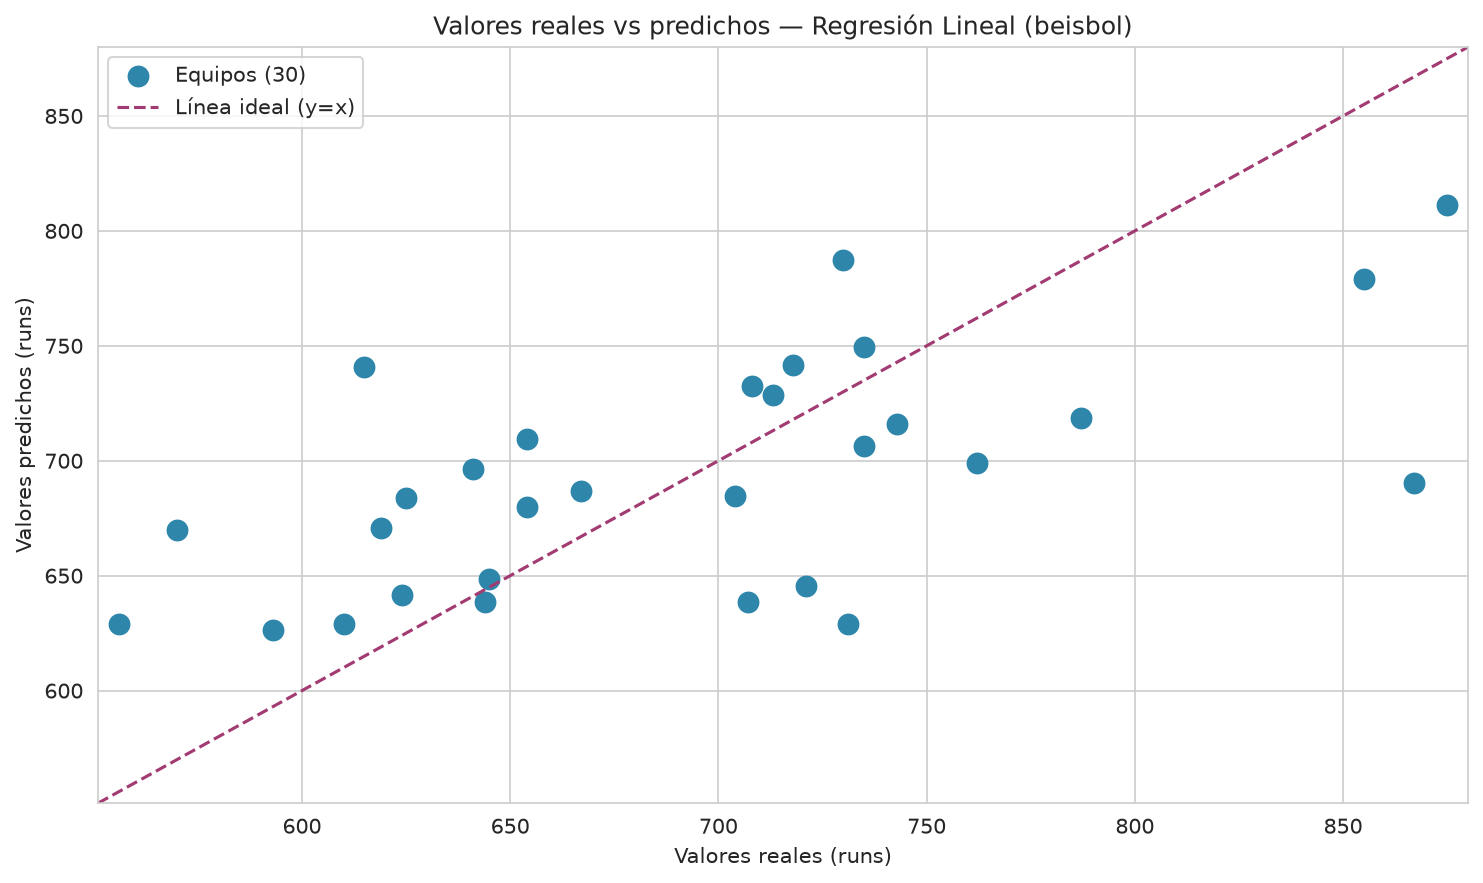
\includegraphics[width=0.82\linewidth]{img/reales_predichos_beisbol.png}
\caption{Valores reales contra predichos. Los puntos se concentran alrededor de la
línea ideal; la dispersión refleja la capacidad predictiva limitada de una sola
variable sobre un conjunto de solo 30 equipos.}
\end{figure}

\textbf{Interpretación.} La regresión lineal explica el 37.3\% de la varianza de las
carreras a partir de los turnos al bat ($R^2=0.3729$), con un error de predicción de
aproximadamente 56--69 carreras según la validación cruzada. La relación es
moderada pero real; el tamaño reducido del conjunto es la principal limitación.

\subsection{Enlace al modelo}
\begin{itemize}
\item Notebook: \url{https://github.com/rmMarioAlberto/evaluacion-u2-extraccion-conocimiento-bd/blob/main/notebooks/1_sa_regresion_lineal.ipynb}
\item Modelo: \url{https://github.com/rmMarioAlberto/evaluacion-u2-extraccion-conocimiento-bd/blob/main/modelos/beisbol_regresion_lineal.pkl}
\end{itemize}

% ================= 3. SA CLASIFICACIÓN =================
\section{Análisis Supervisado 2 — Clasificación sobre breast-cancer.csv}

\subsection{Justificación del algoritmo}
Se eligió el algoritmo de los \textbf{k-Vecinos Más Cercanos (k-NN)} porque el
conjunto tiene 30 características numéricas continuas y una etiqueta binaria
(benigno/maligno). k-NN es un clasificador no paramétrico sencillo e interpretable:
clasifica cada muestra según la mayoría de sus $k$ vecinos más cercanos. Permite una
búsqueda de hiperparámetros clara ($k$, pesos y métrica de distancia) y no asume
linealidad.

\subsection{Diseño del modelo (paso a paso)}
\begin{enumerate}[itemsep=2pt]
\item \textbf{Carga y exploración:} 569 muestras, 30 características, sin nulos;
      balance de clases 357 benignas (B) y 212 malignas (M).
\item \textbf{Preprocesamiento:} se separa la variable objetivo
      (\texttt{diagnosis} $\rightarrow$ 1/0) y se elimina el identificador.
\item \textbf{Particionado:} 75\%/25\% estratificado (\texttt{random\_state=42}).
\item \textbf{Escalado:} \texttt{StandardScaler} ajustado sobre entrenamiento
      (k-NN es sensible a la escala).
\item \textbf{Optimización:} \texttt{GridSearchCV} (5 pliegues) sobre
      $k \in [1,15]$, pesos \texttt{uniform}/\texttt{distance} y métrica
      \texttt{euclidean}/\texttt{manhattan}.
\item \textbf{Entrenamiento final:} k-NN con los mejores hiperparámetros.
\end{enumerate}

\subsection{Evaluación y optimización}
\textbf{Mejores hiperparámetros:} $k=6$, pesos \texttt{distance}, distancia
euclidiana. \textbf{Accuracy en validación cruzada:} 0.9695.

\begin{table}[H]
\centering
\caption{Métricas del clasificador k-NN sobre el conjunto de prueba}
\small\setlength{\tabcolsep}{5pt}\begin{tabular}{lcccc}
\toprule
 & \textbf{Accuracy} & \textbf{Precision} & \textbf{Recall} & \textbf{F1} \\
\midrule
\textbf{k-NN} & 0.9580 & 0.9796 & 0.9057 & 0.9412 \\
\bottomrule
\end{tabular}
\end{table}

\begin{table}[H]
\centering
\caption{Reporte de clasificación por clase}
\small\setlength{\tabcolsep}{5pt}\begin{tabular}{lcccc}
\toprule
\textbf{Clase} & \textbf{Precision} & \textbf{Recall} & \textbf{F1} & \textbf{Soporte} \\
\midrule
Benigno & 0.95 & 0.99 & 0.97 & 90 \\
Maligno & 0.98 & 0.91 & 0.94 & 53 \\
\bottomrule
\end{tabular}
\end{table}

\begin{figure}[H]
\centering
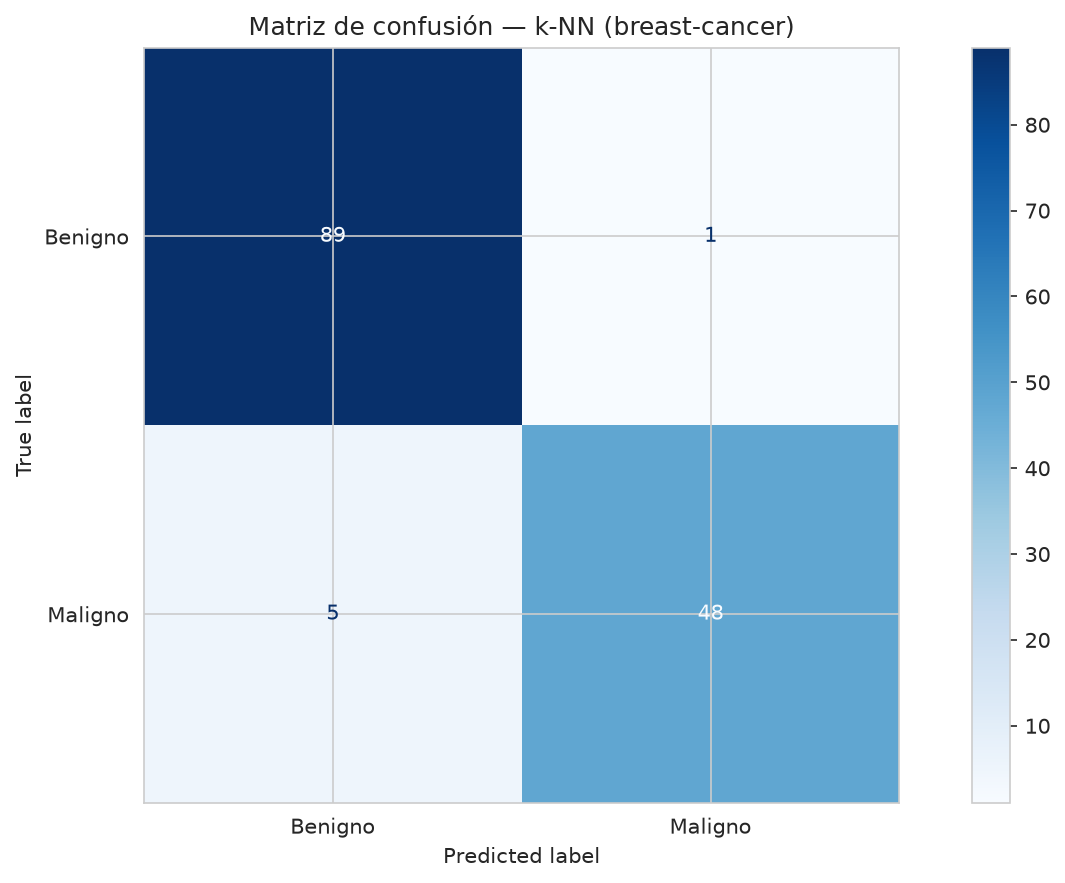
\includegraphics[width=0.72\linewidth]{img/confusion_knn.png}
\caption{Matriz de confusión del clasificador k-NN (test).}
\end{figure}

\begin{figure}[H]
\centering
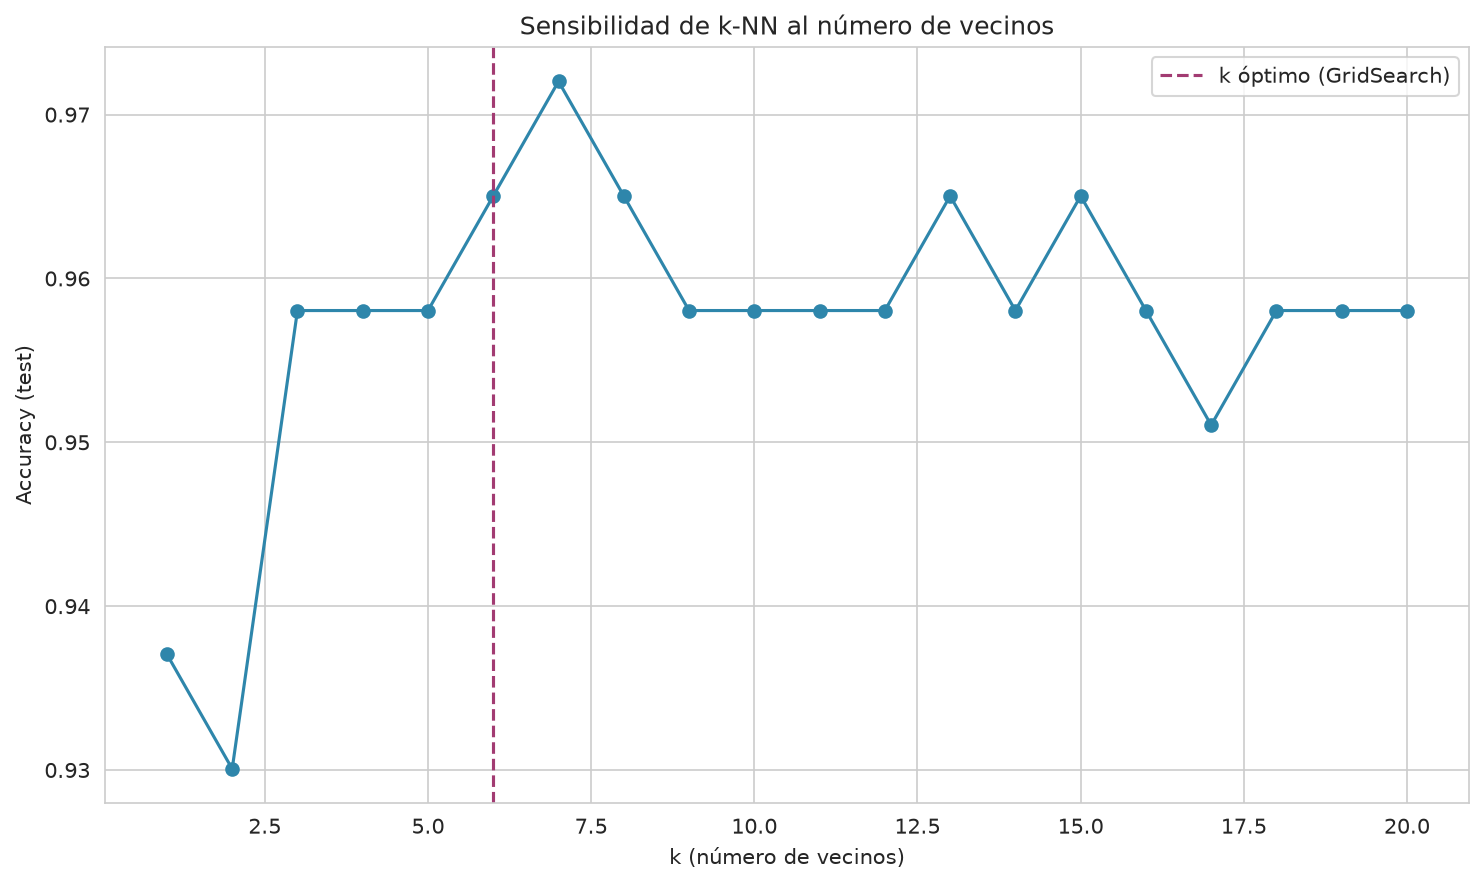
\includegraphics[width=0.82\linewidth]{img/curva_k_knn.png}
\caption{Análisis de sensibilidad al número de vecinos $k$. El accuracy es máximo
cerca de $k=6$ (línea punteada), valor elegido por el GridSearch.}
\end{figure}

\begin{figure}[H]
\centering
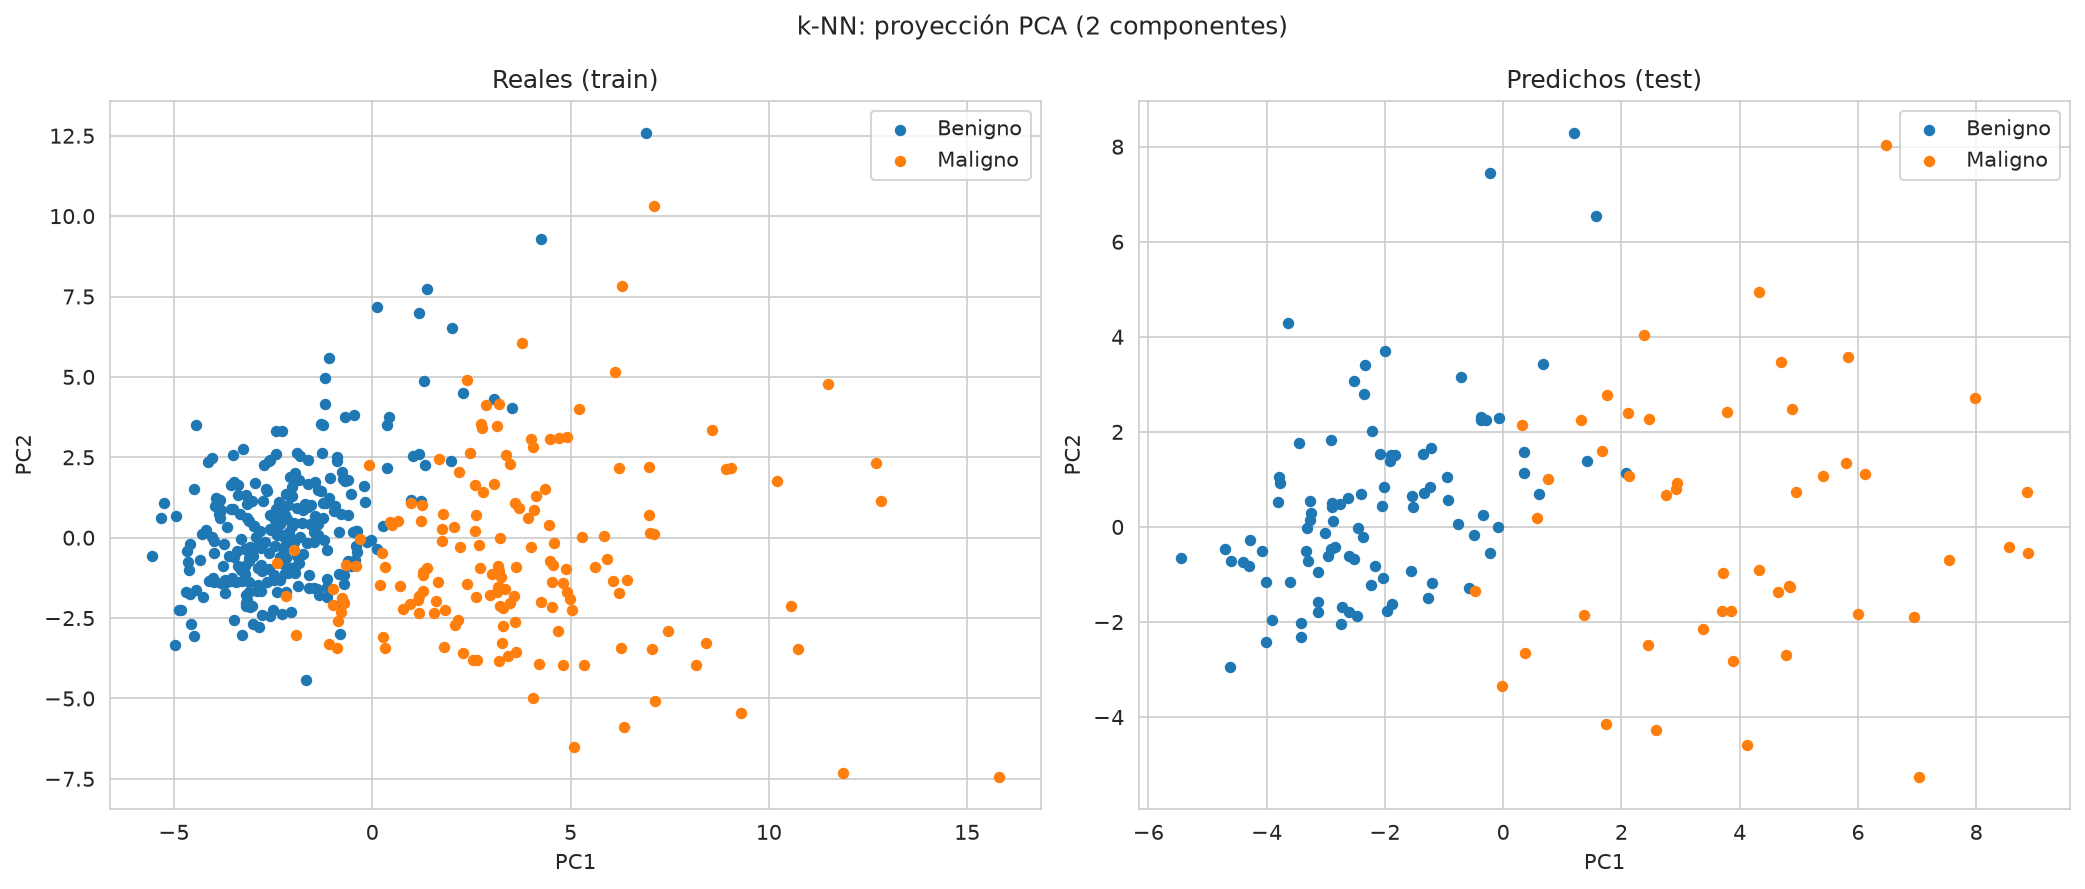
\includegraphics[width=0.95\linewidth]{img/pca_knn_classes.png}
\caption{Proyección PCA (2 componentes) de las clases reales (train) y predichas
(test). Se aprecia una separación clara entre benignos y malignos.}
\end{figure}

\subsection{Enlace al modelo}
\begin{itemize}
\item Notebook: \url{https://github.com/rmMarioAlberto/evaluacion-u2-extraccion-conocimiento-bd/blob/main/notebooks/2_sa_clasificacion_knn.ipynb}
\item Modelo: \url{https://github.com/rmMarioAlberto/evaluacion-u2-extraccion-conocimiento-bd/blob/main/modelos/breast_knn.pkl}
\end{itemize}

% ================= 4. NS AGRUPACIÓN =================
\section{Análisis No Supervisado 3 — Agrupación sobre samsung.csv}

\subsection{Justificación del algoritmo}
Se eligió \textbf{K-Means} porque se busca particionar las observaciones (días de
cotización) en grupos homogéneos a partir de características numéricas continuas, sin
etiquetas previas. Es el algoritmo de agrupación más utilizado por su sencillez y
eficiencia. El número de clusters $k$ se optimizó con el \textbf{método del codo}
(inercia), el \textbf{coeficiente de silueta} y el índice de \textbf{Davies-Bouldin}.

\subsection{Diseño del modelo (paso a paso)}
\begin{enumerate}[itemsep=2pt]
\item \textbf{Carga y exploración:} 2,850 días (2008--2019) con precio de cierre
      (\texttt{Close}) y volumen (\texttt{Volume}).
\item \textbf{Ingeniería de características:} retorno diario (\%), volumen
      logarítmico y medias móviles de 5 y 20 días; se descartan filas con NaN
      (quedan 2,831 observaciones).
\item \textbf{Escalado:} \texttt{StandardScaler} sobre las 6 características.
\item \textbf{Optimización de $k$:} para $k=2,\dots,10$ se calculan inercia,
      silueta y Davies-Bouldin.
\item \textbf{Entrenamiento final:} K-Means con el $k$ óptimo.
\end{enumerate}

\subsection{Optimización del número de clusters}
\begin{table}[H]
\centering
\caption{Métricas de evaluación para cada $k$}
\begin{tabular}{cccc}
\toprule
$k$ & \textbf{Inercia} & \textbf{Silueta} & \textbf{Davies-Bouldin} \\
\midrule
2 & 10604.48 & \textbf{0.4510} & \textbf{0.7953} \\
3 & 7935.45 & 0.3794 & 1.0393 \\
4 & 5619.45 & 0.3916 & 0.8201 \\
5 & 4545.44 & 0.3933 & 0.8592 \\
6 & 3848.05 & 0.3818 & 0.8339 \\
7 & 3442.56 & 0.3330 & 0.8964 \\
8 & 3193.31 & 0.3409 & 0.8630 \\
9 & 2947.50 & 0.3010 & 1.0045 \\
10 & 2741.43 & 0.2866 & 1.0652 \\
\bottomrule
\end{tabular}
\end{table}

\begin{figure}[H]
\centering
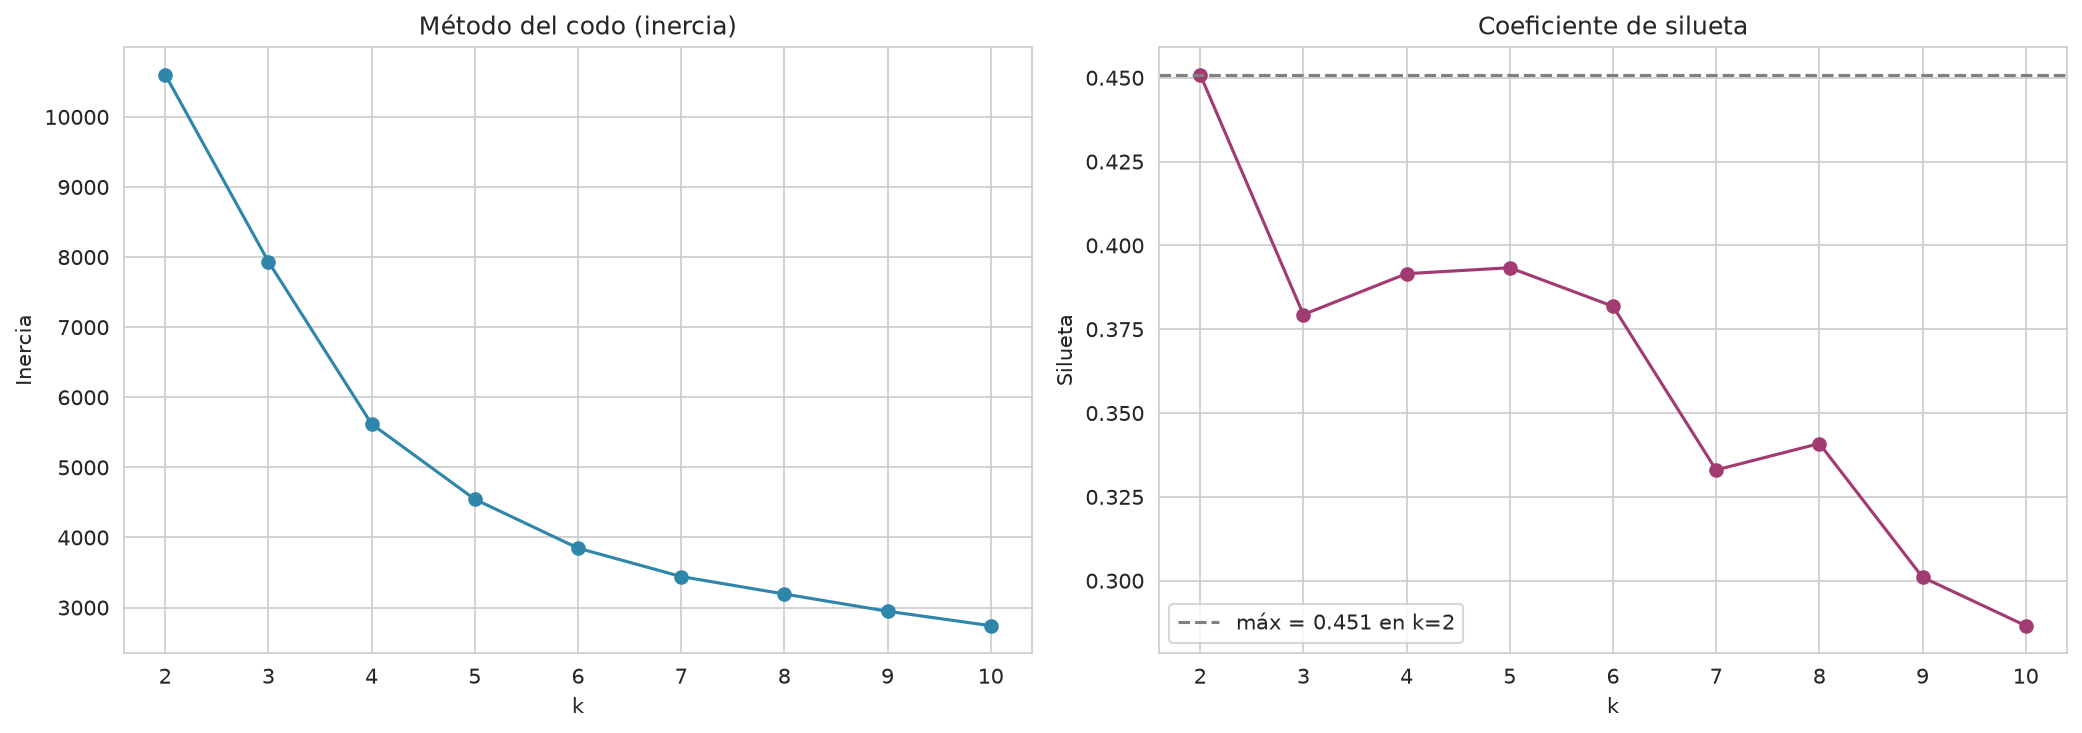
\includegraphics[width=0.95\linewidth]{img/elbow_silhouette_samsung.png}
\caption{Método del codo (inercia) y coeficiente de silueta para $k=2,\dots,10$. La
silueta es máxima en $k=2$ (0.4510).}
\end{figure}

\textbf{Selección de $k$:} el coeficiente de silueta y el índice de Davies-Bouldin
coinciden en que el mejor número de clusters es $\mathbf{k=2}$.

\subsection{Gráficas e interpretación de resultados}
\begin{figure}[H]
\centering
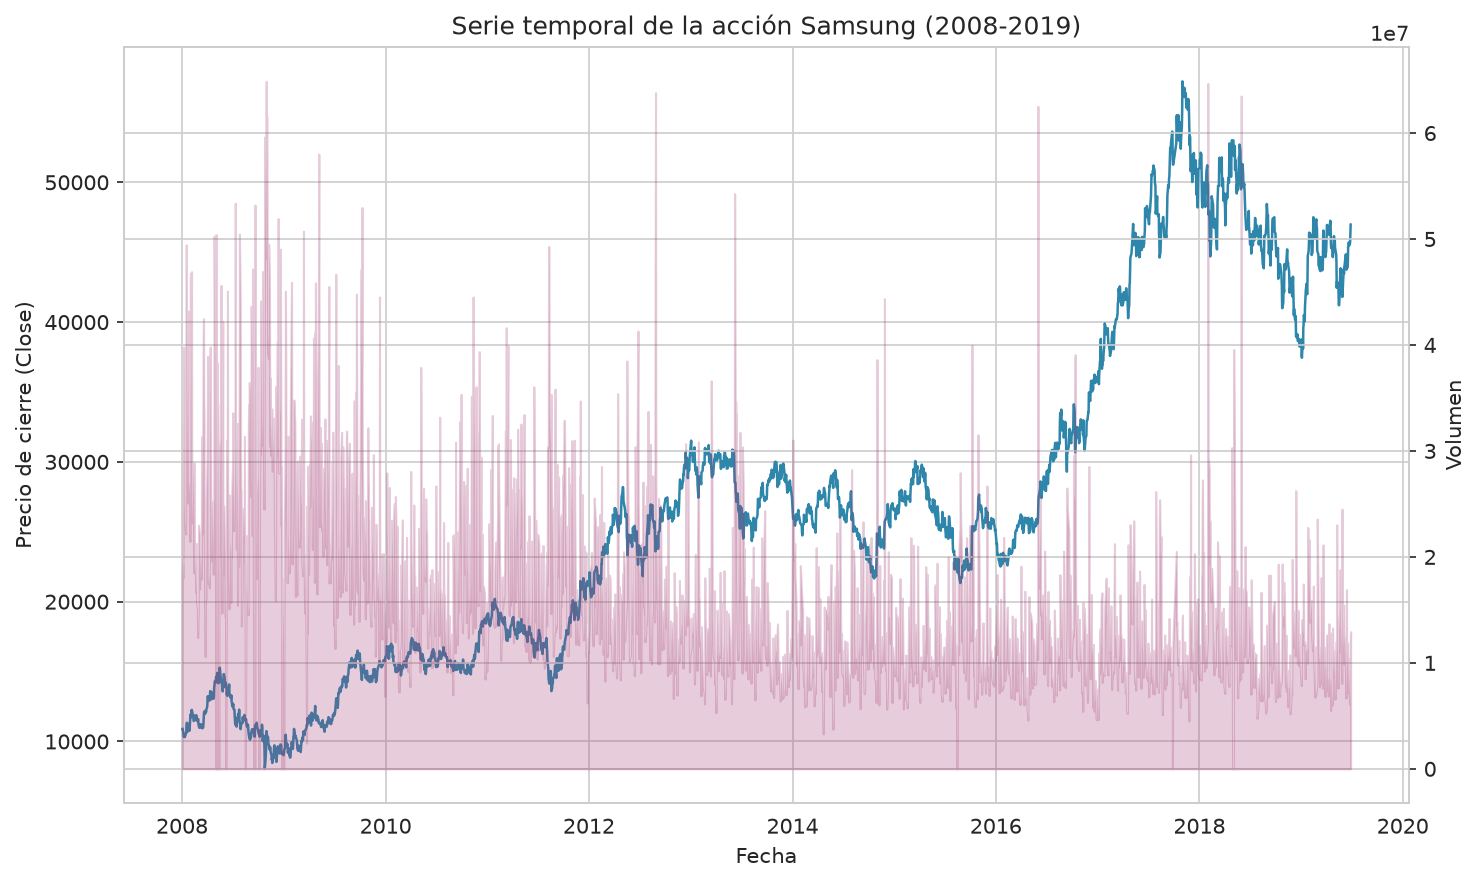
\includegraphics[width=0.95\linewidth]{img/serie_samsung.png}
\caption{Serie temporal del precio (línea) y volumen (área) de la acción Samsung.}
\end{figure}

\begin{figure}[H]
\centering
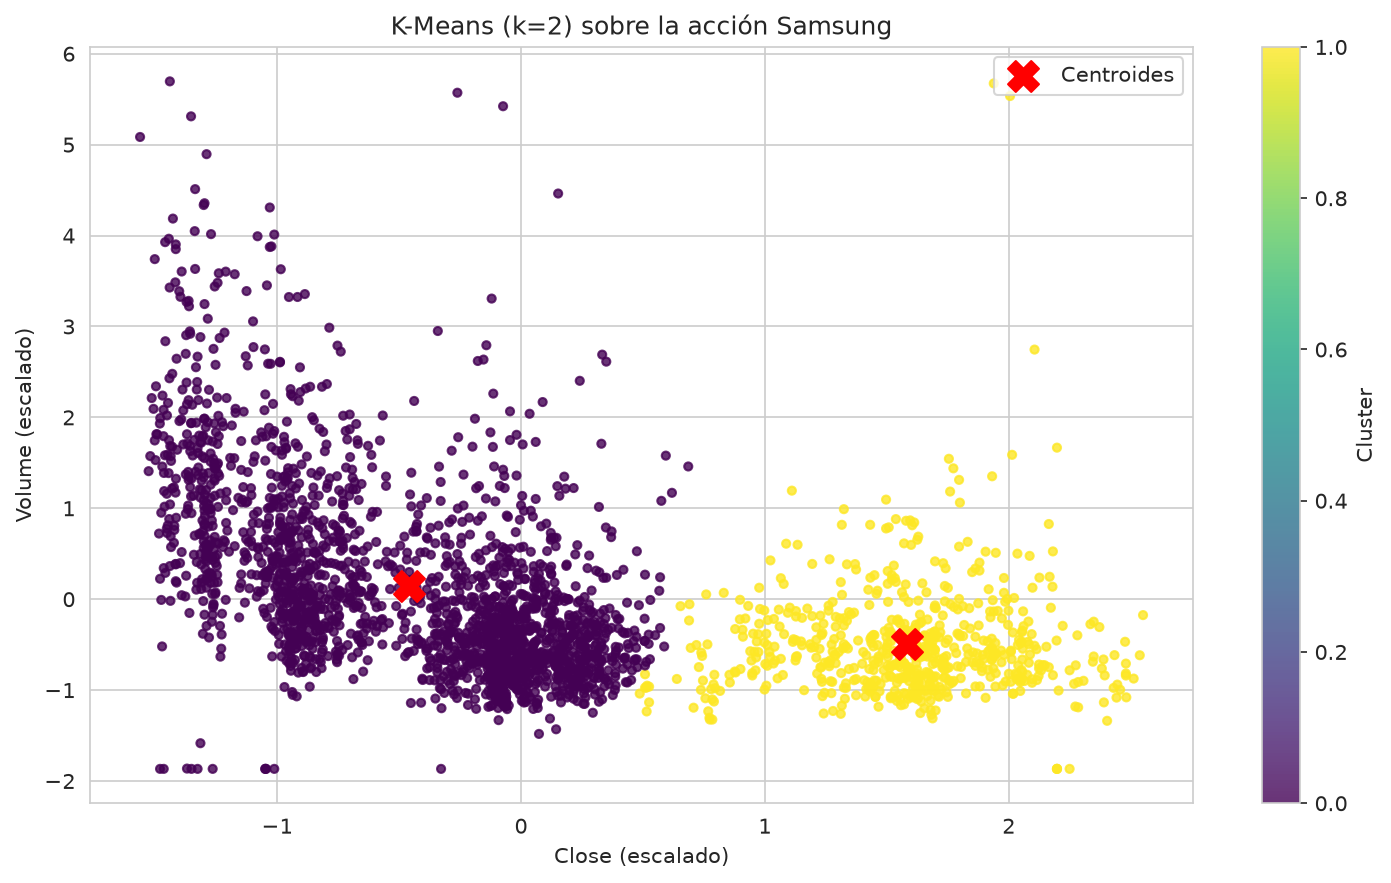
\includegraphics[width=0.82\linewidth]{img/clusters_samsung.png}
\caption{Clusters obtenidos por K-Means ($k=2$) sobre las características
escaladas; los centroides se marcan con X.}
\end{figure}

\begin{figure}[H]
\centering
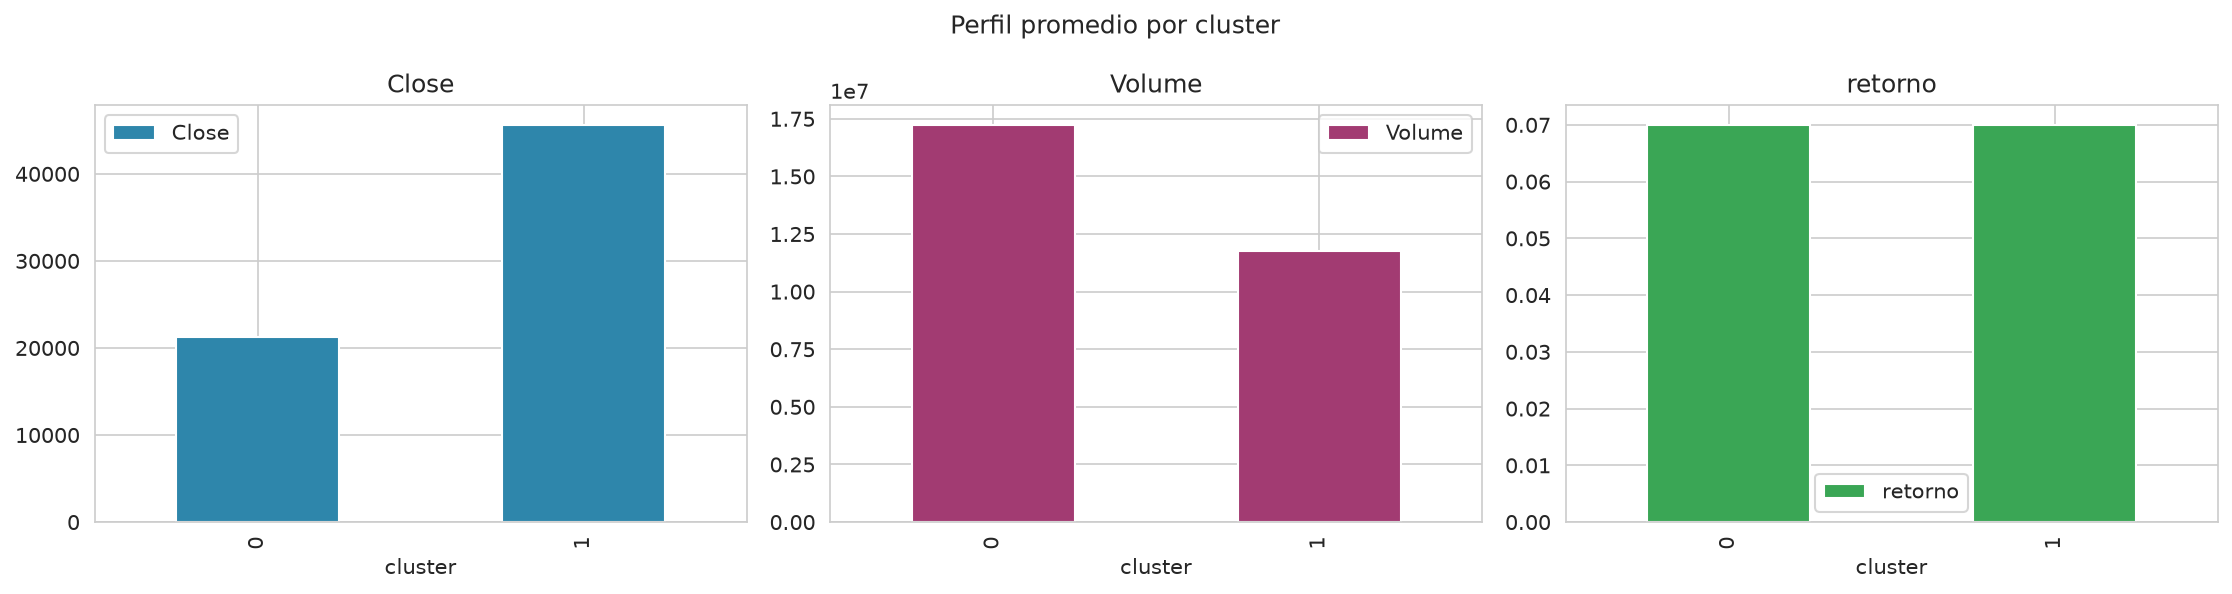
\includegraphics[width=0.95\linewidth]{img/perfil_clusters_samsung.png}
\caption{Perfil promedio de cada cluster.}
\end{figure}

\textbf{Interpretación.} El cluster 0 (2,196 días) agrupa días con precio medio de
$\approx 21{,}249$ y volumen alto ($\approx 17.2$ millones); el cluster 1 (635 días)
agrupa días con precio medio de $\approx 45{,}631$ y volumen menor
($\approx 11.8$ millones). Es decir, los clusters separan \emph{periodos de precio
bajo-alto volumen} de \emph{periodos de precio alto-bajo volumen}, revelando dos
regímenes de mercado distintos.

\subsection{Enlace al modelo}
\begin{itemize}
\item Notebook: \url{https://github.com/rmMarioAlberto/evaluacion-u2-extraccion-conocimiento-bd/blob/main/notebooks/3_ns_agrupacion_kmeans.ipynb}
\item Modelo: \url{https://github.com/rmMarioAlberto/evaluacion-u2-extraccion-conocimiento-bd/blob/main/modelos/samsung_kmeans.pkl}
\end{itemize}

% ================= 5. NS REDUCCIÓN =================
\section{Análisis No Supervisado 4 — Reducción de dimensionalidad sobre comprar\_alquilar.csv}

\subsection{Justificación del algoritmo}
Se eligió \textbf{Análisis de Componentes Principales (PCA)}, el método de
reducción de dimensionalidad más estándar: proyecta los datos a direcciones
ortogonales que capturan la mayor varianza posible. Permite visualizar 9 variables
predictoras en 2D, elimina redundancia y facilita modelos posteriores. La elección
del número de componentes se justificó con la \textbf{varianza explicada acumulada}
(umbral del 95\%) y el criterio de \textbf{Kaiser} (autovalores $>1$).

\subsection{Diseño del modelo (paso a paso)}
\begin{enumerate}[itemsep=2pt]
\item \textbf{Carga y exploración:} 202 registros, 9 variables predictoras y la
      variable objetivo \texttt{comprar}.
\item \textbf{Comparación sin/con escalado:} se calcula PCA con 2 componentes sobre
      los datos brutos y sobre los datos estandarizados.
\item \textbf{Justificación del número de componentes:} se ajusta PCA completo y se
      calculan la varianza explicada y su acumulada.
\item \textbf{Reducción final:} proyección con el número de componentes que captura
      al menos el 95\% de la varianza.
\end{enumerate}

\subsection{Comparación de los dos primeros componentes}
\begin{figure}[H]
\centering
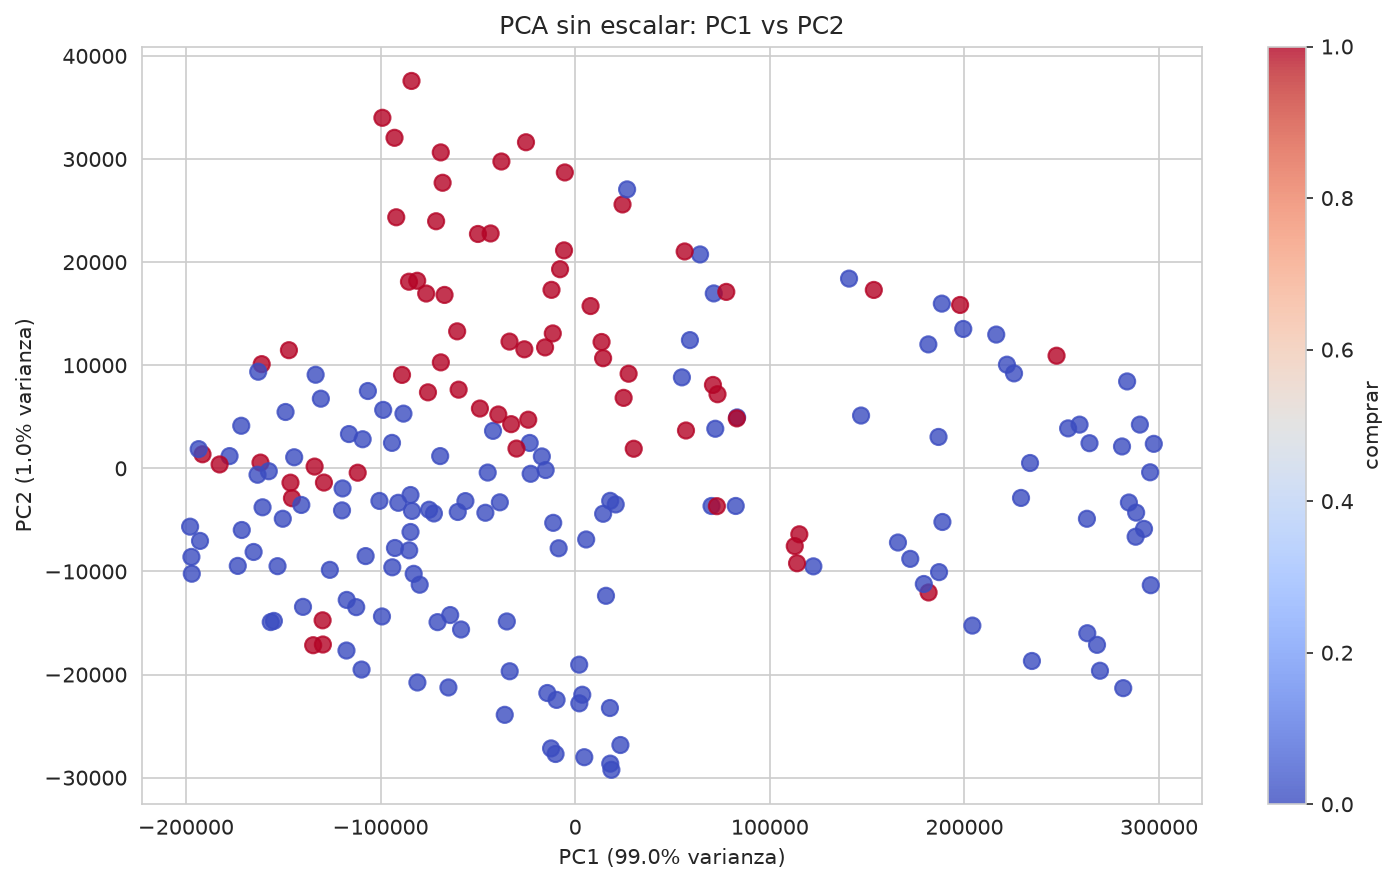
\includegraphics[width=0.82\linewidth]{img/pca_sin_escalado.png}
\caption{PCA sin escalado: PC1 concentra el 99\% de la varianza porque las variables
de mayor magnitud (p.~ej. \texttt{vivienda}, desviación 136,371) dominan.}
\end{figure}

\begin{figure}[H]
\centering
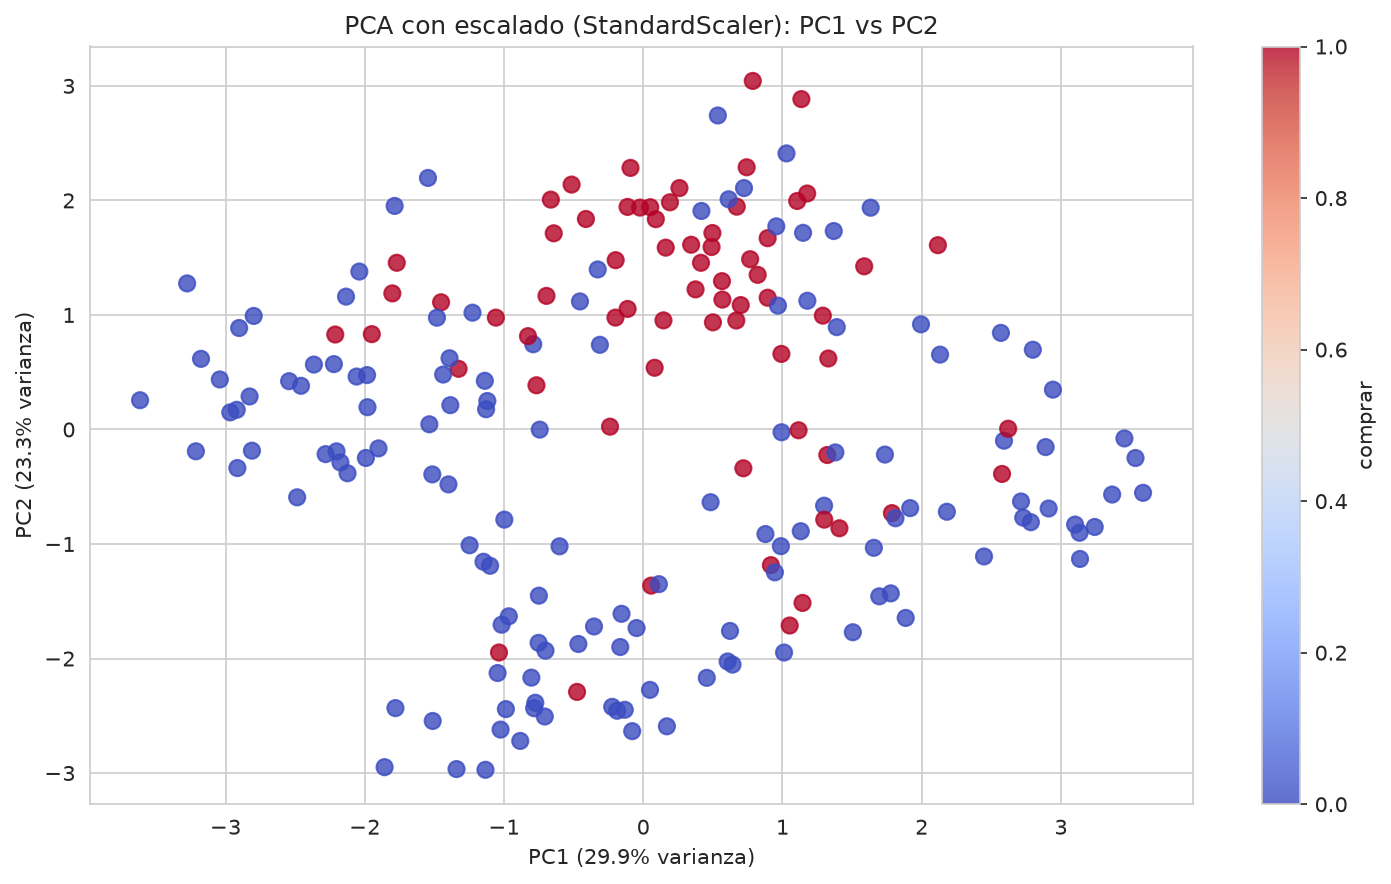
\includegraphics[width=0.82\linewidth]{img/pca_con_escalado.png}
\caption{PCA con escalado (\texttt{StandardScaler}): PC1 (29.9\%) y PC2 (23.3\%)
distribuyen mejor la varianza entre todas las variables.}
\end{figure}

\textbf{Importancia del escalado:} sin escalar, PC1 explica el 99\% de la varianza
porque queda dominada por \texttt{vivienda}; con escalado, PC1 y PC2 explican 29.9\%
y 23.3\%, respectivamente, y todos los puntos se distribuyen de forma más
informativa. Por eso el análisis final usa datos escalados.

\subsection{Justificación del número de componentes}
\begin{table}[H]
\centering
\caption{Varianza explicada (PCA con escalado)}
\small\setlength{\tabcolsep}{5pt}\begin{tabular}{ccccc}
\toprule
\textbf{Componente} & \textbf{Varianza} & \textbf{Acumulada} &
\textbf{Componente} & \textbf{Varianza acumulada} \\
\midrule
1 & 0.299 & 0.299 & 6 & 0.909 \\
2 & 0.233 & 0.532 & 7 & \textbf{0.950} \\
3 & 0.117 & 0.649 & 8 & 0.980 \\
4 & 0.107 & 0.756 & 9 & 1.000 \\
5 & 0.096 & 0.852 & & \\
\bottomrule
\end{tabular}
\end{table}

\begin{figure}[H]
\centering
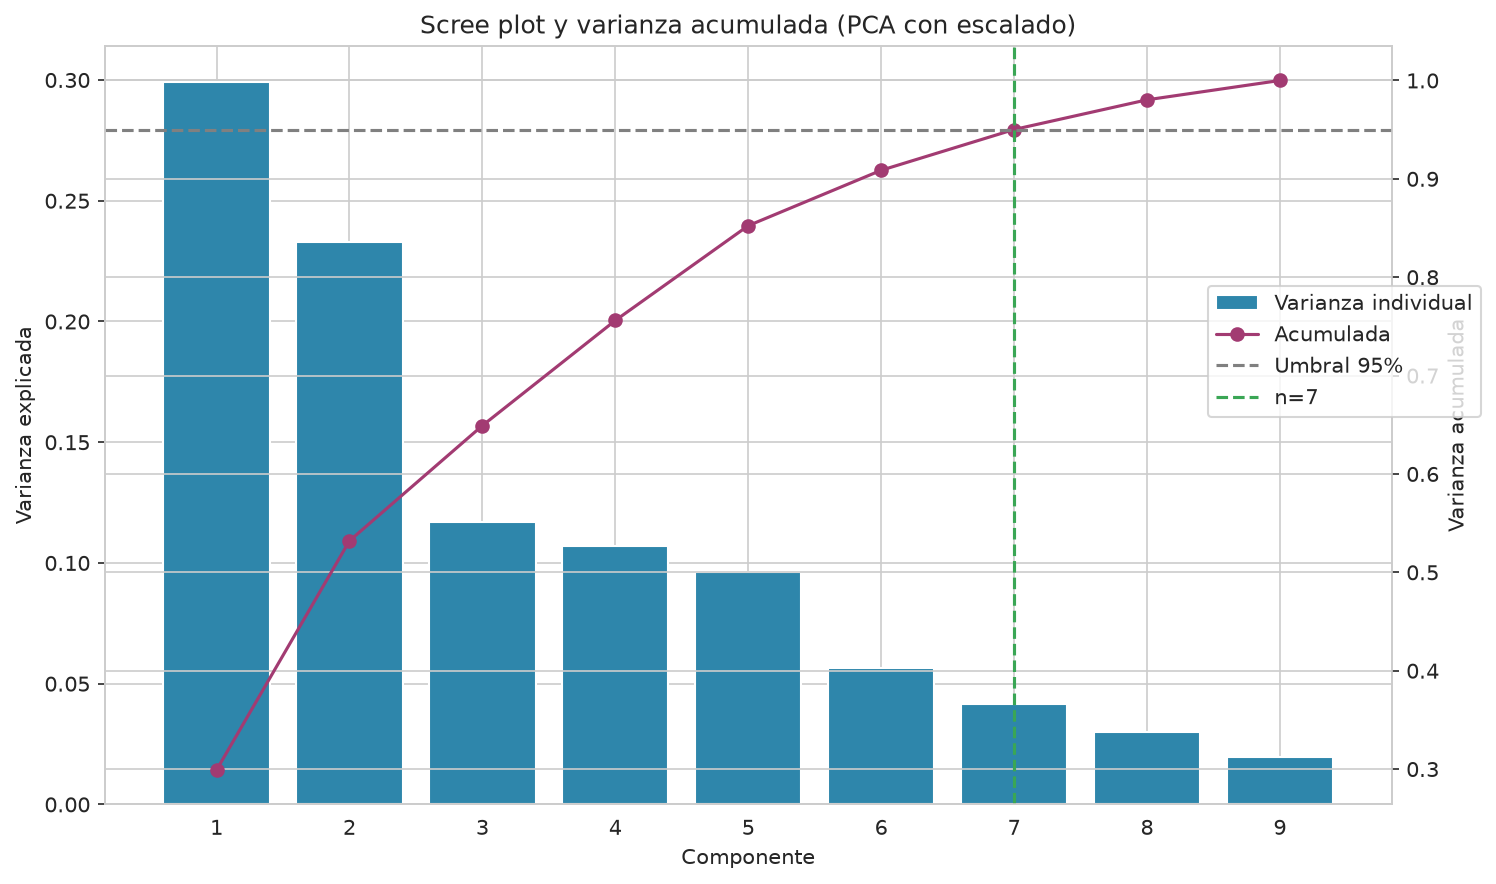
\includegraphics[width=0.85\linewidth]{img/varianza_pca.png}
\caption{Scree plot y varianza acumulada. Se requieren 7 componentes para alcanzar
el umbral del 95\%.}
\end{figure}

\textbf{Decisión:} se eligen $\mathbf{n=7}$ componentes, que capturan el 95.02\% de
la varianza total, reduciendo los datos de 9 a 7 dimensiones. (El criterio de Kaiser
sugiere 3 componentes por autovalor $>1$; el umbral del 95\% es la elección
adoptada por ser el más común en la práctica.)

\begin{figure}[H]
\centering
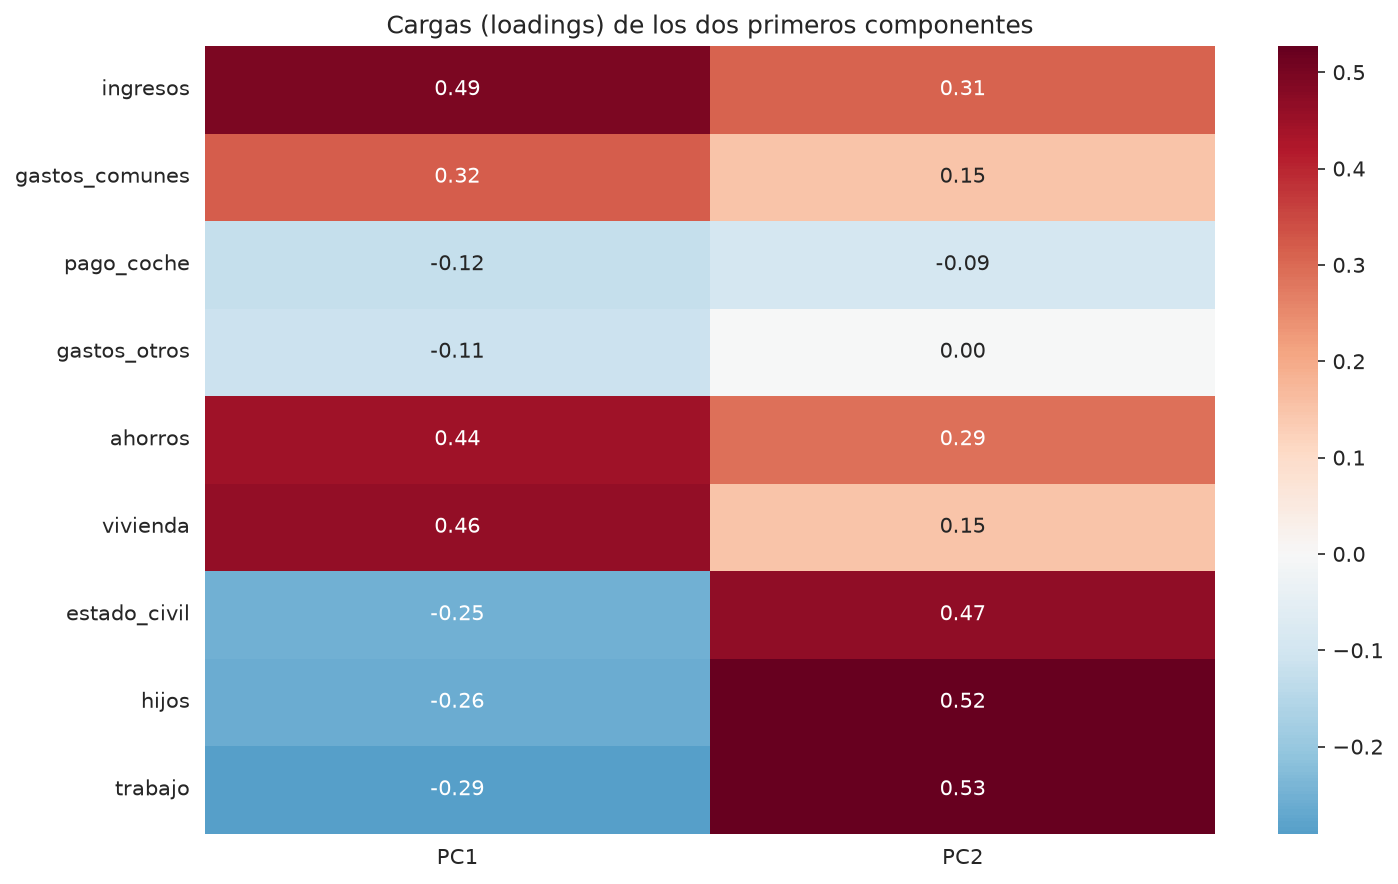
\includegraphics[width=0.85\linewidth]{img/loadings_pca.png}
\caption{Cargas (loadings) de los dos primeros componentes: muestran qué variables
contribuyen más a cada componente.}
\end{figure}

\subsection{Enlace al modelo}
\begin{itemize}
\item Notebook: \url{https://github.com/rmMarioAlberto/evaluacion-u2-extraccion-conocimiento-bd/blob/main/notebooks/4_ns_pca.ipynb}
\item Modelo: \url{https://github.com/rmMarioAlberto/evaluacion-u2-extraccion-conocimiento-bd/blob/main/modelos/comprar_alquilar_pca.pkl}
\end{itemize}

% ================= 6. DE =================
\section{Evaluación DE — Algoritmos alternos a SA}

La evaluación DE solicita implementar un algoritmo de clasificación y uno de
regresión \emph{distintos} a los usados en SA, sobre los mismos conjuntos de datos.

\subsection{DE 1 — Clasificación con Random Forest}

\subsubsection{Justificación del algoritmo}
Se eligió \textbf{Random Forest} como alterno al k-NN de SA. Es un ensamble de
árboles de decisión (bagging) que reduce la varianza y el sobreajuste, maneja bien
datos tabulares con muchas características y no requiere escalado. Permite además
medir la importancia de las características.

\subsubsection{Diseño, evaluación y optimización}
\textbf{Hiperparámetros óptimos (GridSearchCV):} $n\_estimators=100$,
$max\_depth=$ sin límite, $min\_samples\_split=2$. Accuracy en CV: 0.9648.

\begin{table}[H]
\centering
\caption{Métricas de Random Forest sobre el conjunto de prueba}
\small\setlength{\tabcolsep}{5pt}\begin{tabular}{lcccc}
\toprule
 & \textbf{Accuracy} & \textbf{Precision} & \textbf{Recall} & \textbf{F1} \\
\midrule
\textbf{Random Forest} & 0.9650 & 1.0000 & 0.9057 & 0.9505 \\
\textbf{k-NN (SA)} & 0.9580 & 0.9796 & 0.9057 & 0.9412 \\
\bottomrule
\end{tabular}
\end{table}

\begin{figure}[H]
\centering
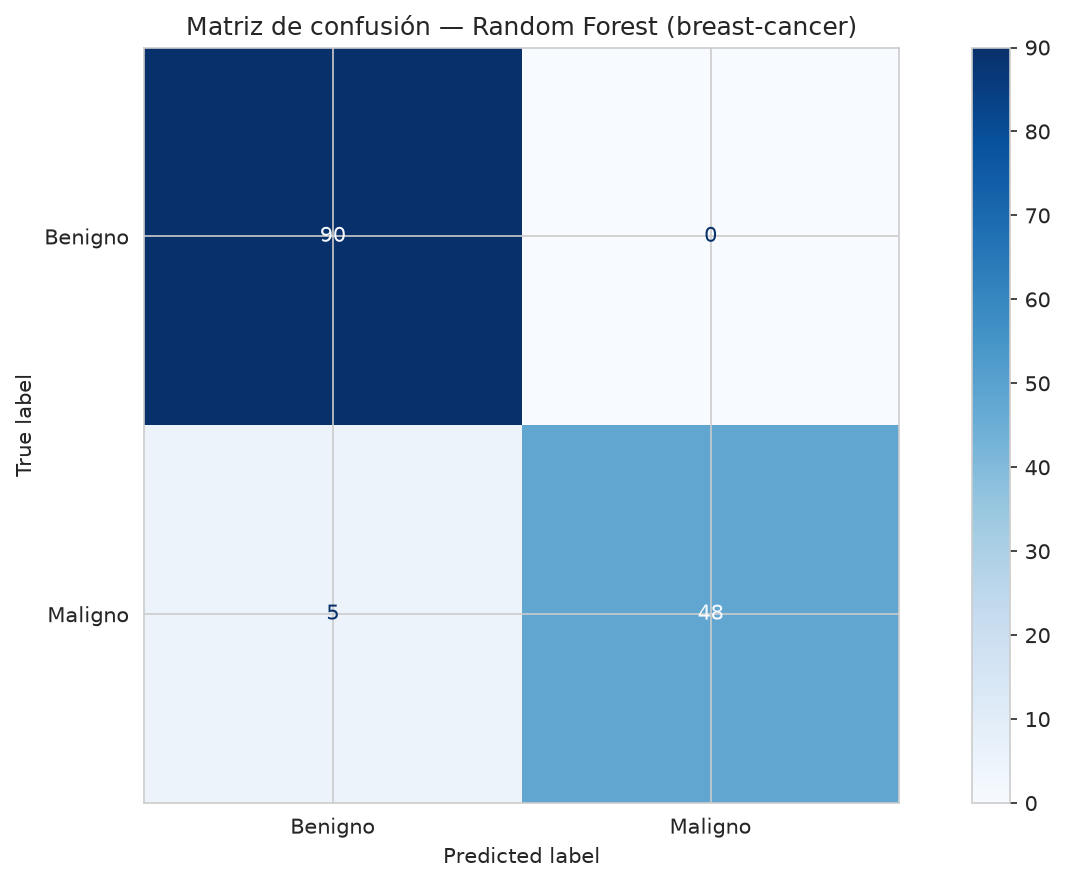
\includegraphics[width=0.72\linewidth]{img/confusion_rf.png}
\caption{Matriz de confusión del Random Forest (test).}
\end{figure}

\begin{figure}[H]
\centering
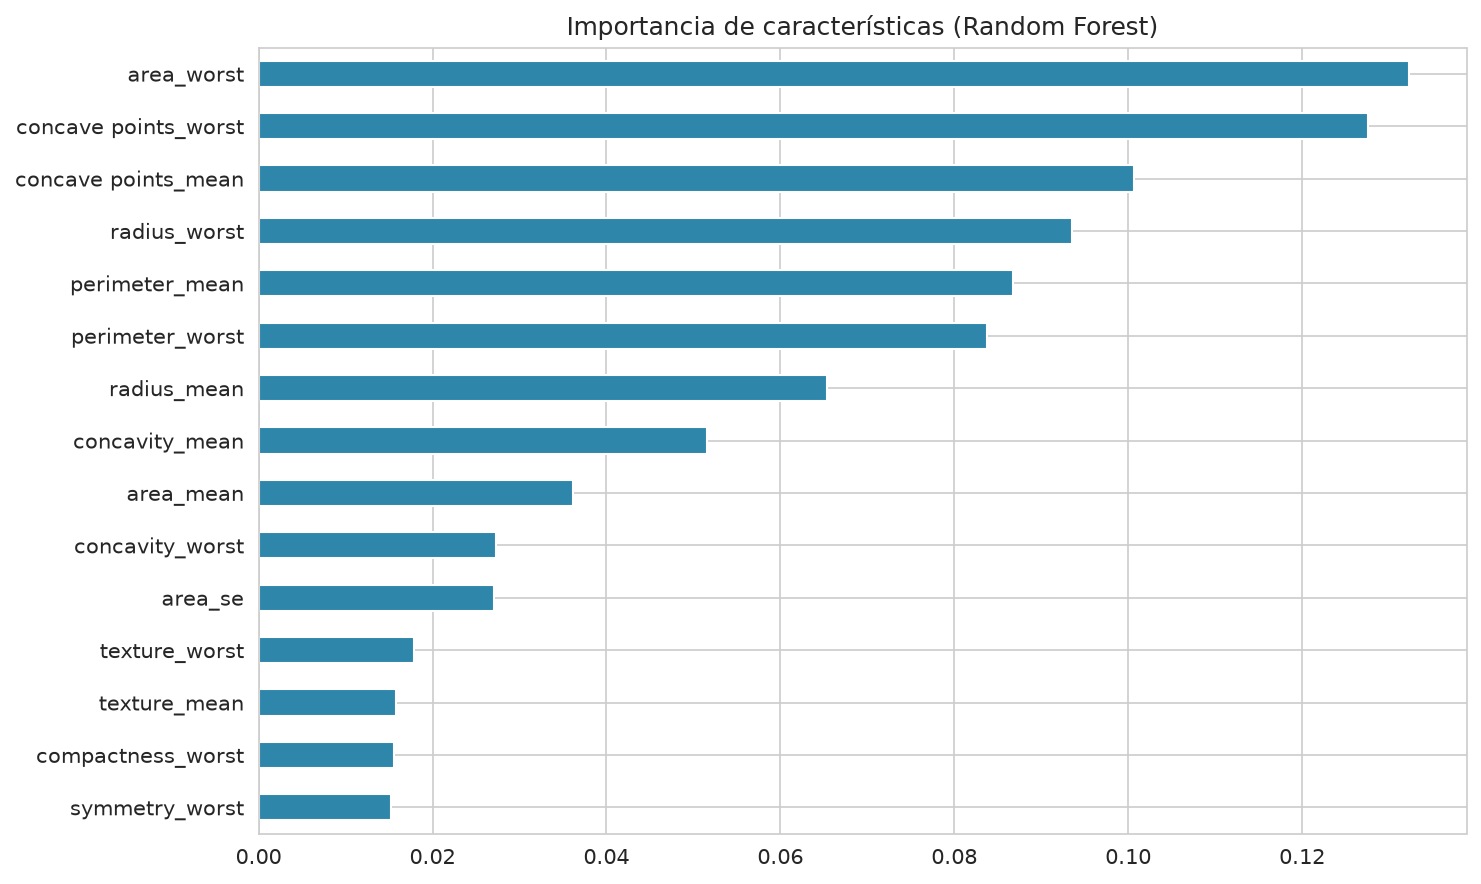
\includegraphics[width=0.8\linewidth]{img/importancia_rf.png}
\caption{Importancia de las características: las más relevantes son
\texttt{worst\_area}, \texttt{worst\_concave\_points} y \texttt{worst\_perimeter}.}
\end{figure}

\begin{figure}[H]
\centering
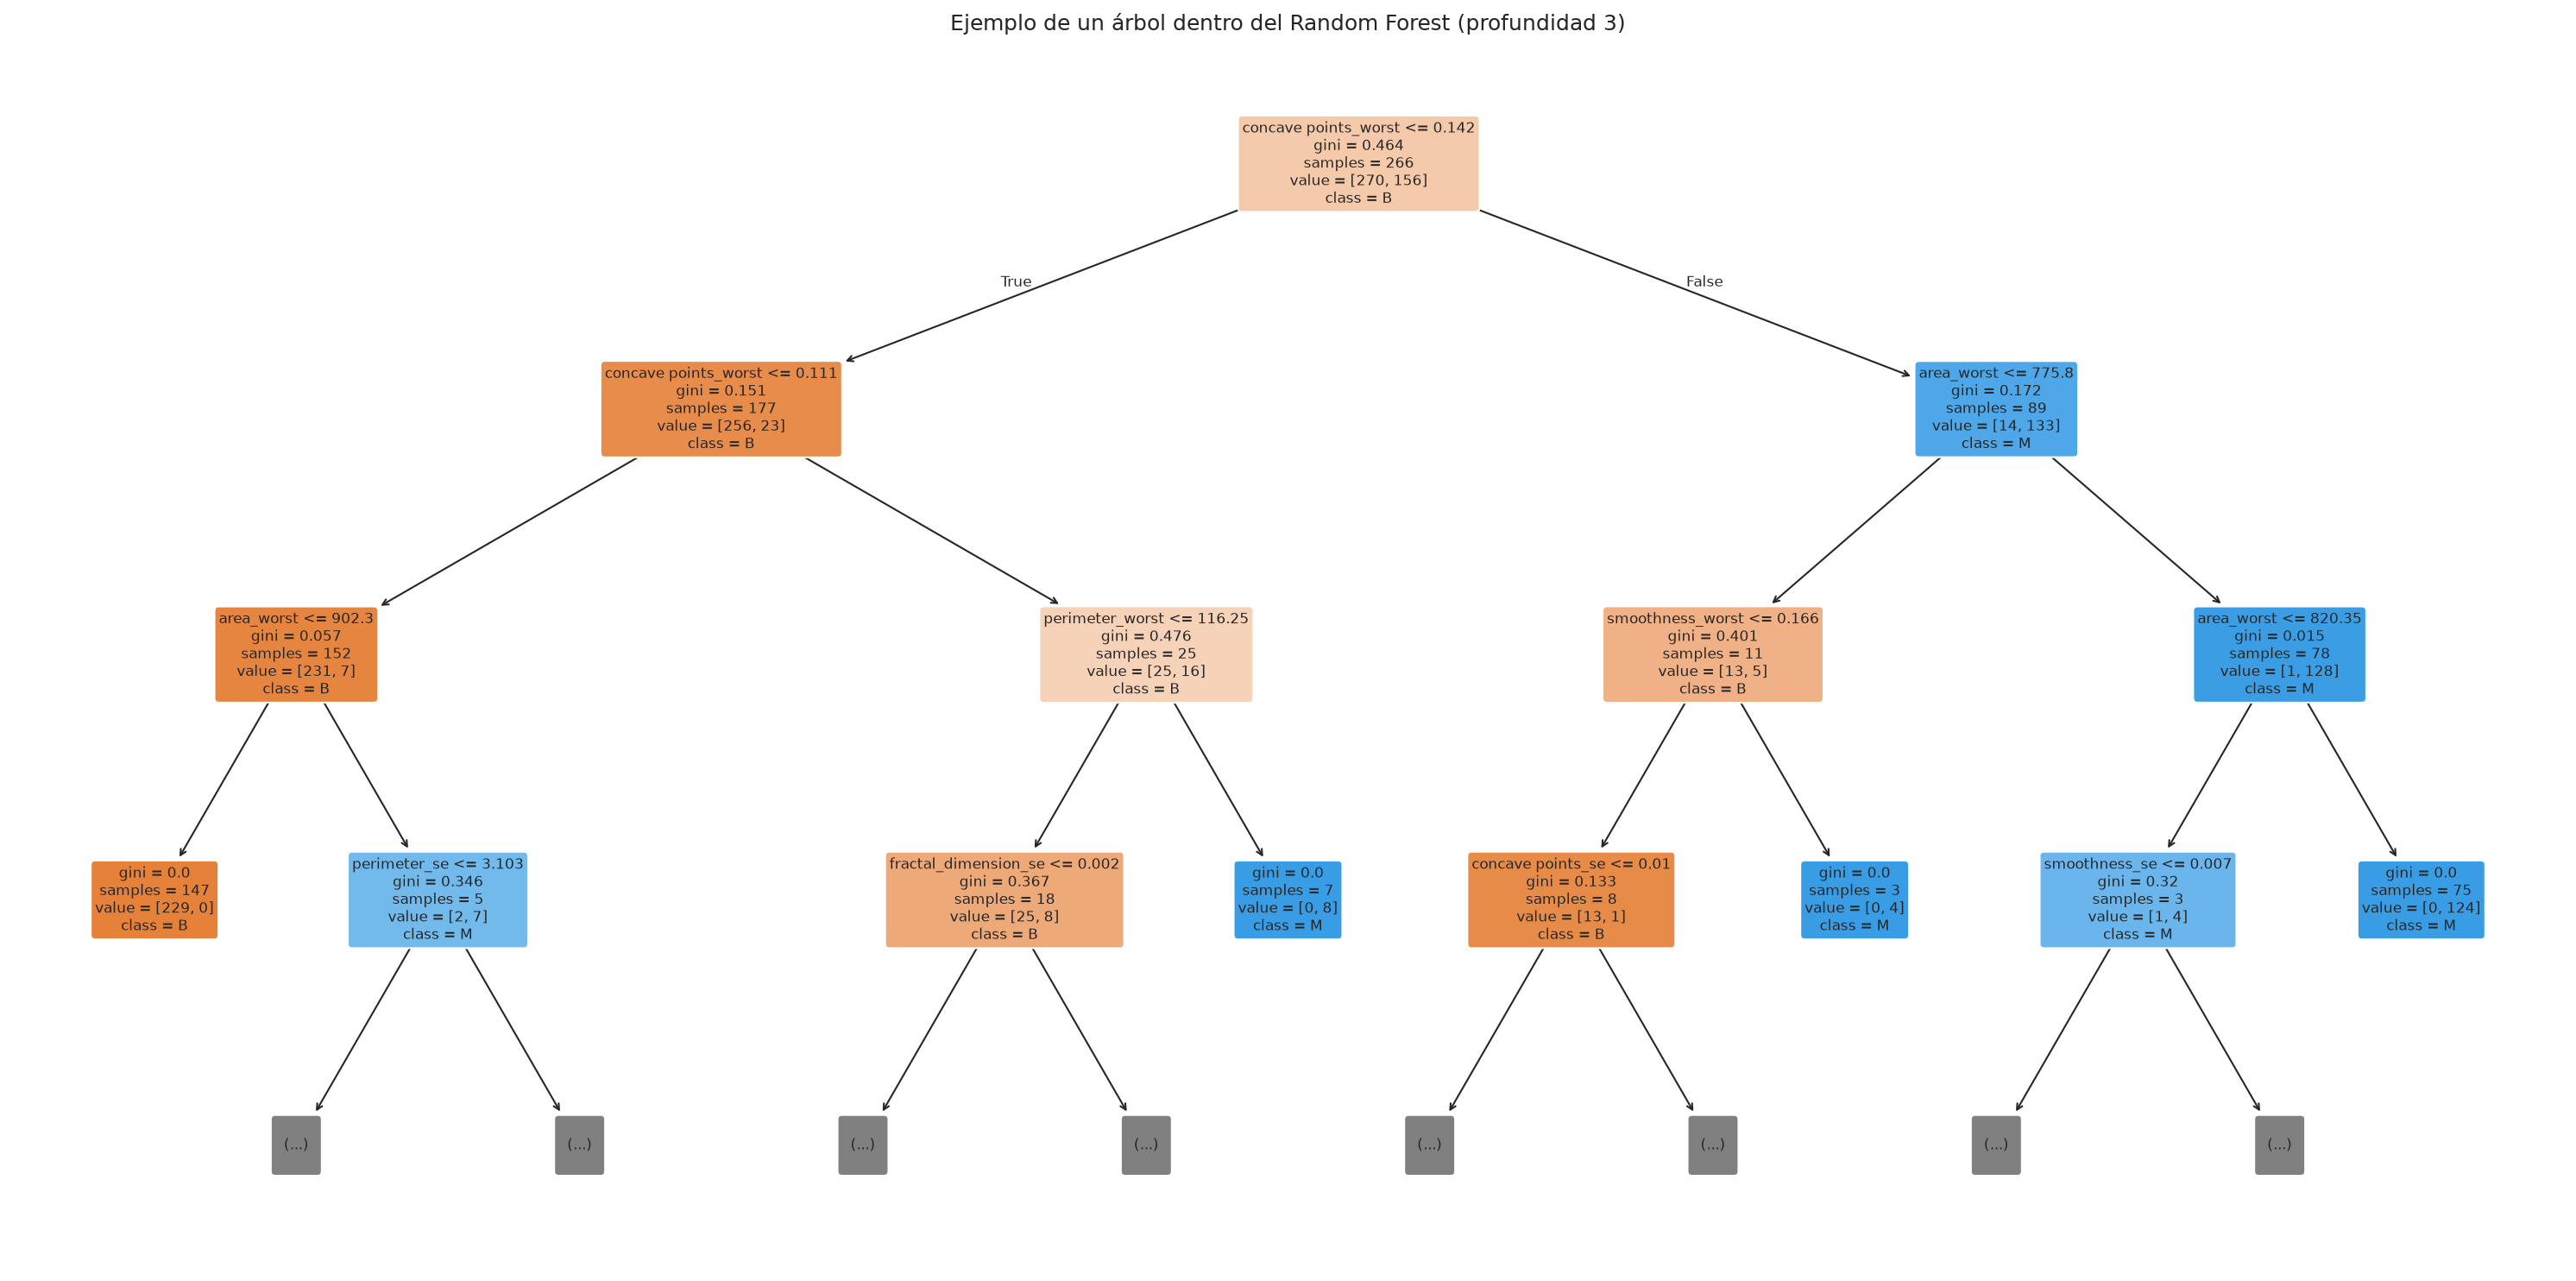
\includegraphics[width=0.95\linewidth]{img/arbol_rf.png}
\caption{Ejemplo de un árbol dentro del bosque (profundidad 3) graficado con
\texttt{plot\_tree}.}
\end{figure}

\textbf{Enlace al modelo:}
\begin{itemize}
\item Notebook: \url{https://github.com/rmMarioAlberto/evaluacion-u2-extraccion-conocimiento-bd/blob/main/notebooks/5_de_clasificacion_randomforest.ipynb}
\item Modelo: \url{https://github.com/rmMarioAlberto/evaluacion-u2-extraccion-conocimiento-bd/blob/main/modelos/breast_randomforest.pkl}
\end{itemize}

\subsection{DE 2 — Regresión con Random Forest}

\subsubsection{Justificación del algoritmo}
Se eligió \textbf{Random Forest Regressor} como alterno a la regresión lineal de
SA. Al ser un ensamble de árboles, puede capturar relaciones no lineales entre
\texttt{bateos} y \texttt{runs} sin asumir una forma paramétrica.

\subsubsection{Diseño, evaluación y optimización}
\textbf{Hiperparámetros óptimos (GridSearchCV):} $n\_estimators=50$,
$max\_depth=$ sin límite, $min\_samples\_leaf=4$.

\begin{table}[H]
\centering
\caption{Métricas de Random Forest Regressor (ajuste completo)}
\begin{tabular}{lccc}
\toprule
\textbf{Modelo} & $R^2$ & \textbf{RMSE} & \textbf{MAE} \\
\midrule
\textbf{Random Forest} & 0.4060 & 62.50 & 47.53 \\
\textbf{Regresión Lineal (SA)} & 0.3729 & 64.22 & 51.67 \\
\bottomrule
\end{tabular}
\end{table}

\textbf{Validación cruzada (RMSE):} LOOCV = 59.08, 5-fold = 76.27. El Random Forest
obtiene un $R^2$ ligeramente superior al lineal en el ajuste completo, aunque con
validación cruzada su RMSE es comparable o ligeramente mayor, lo que confirma que la
ganancia de complejidad es marginal con tan pocas observaciones.

\begin{figure}[H]
\centering
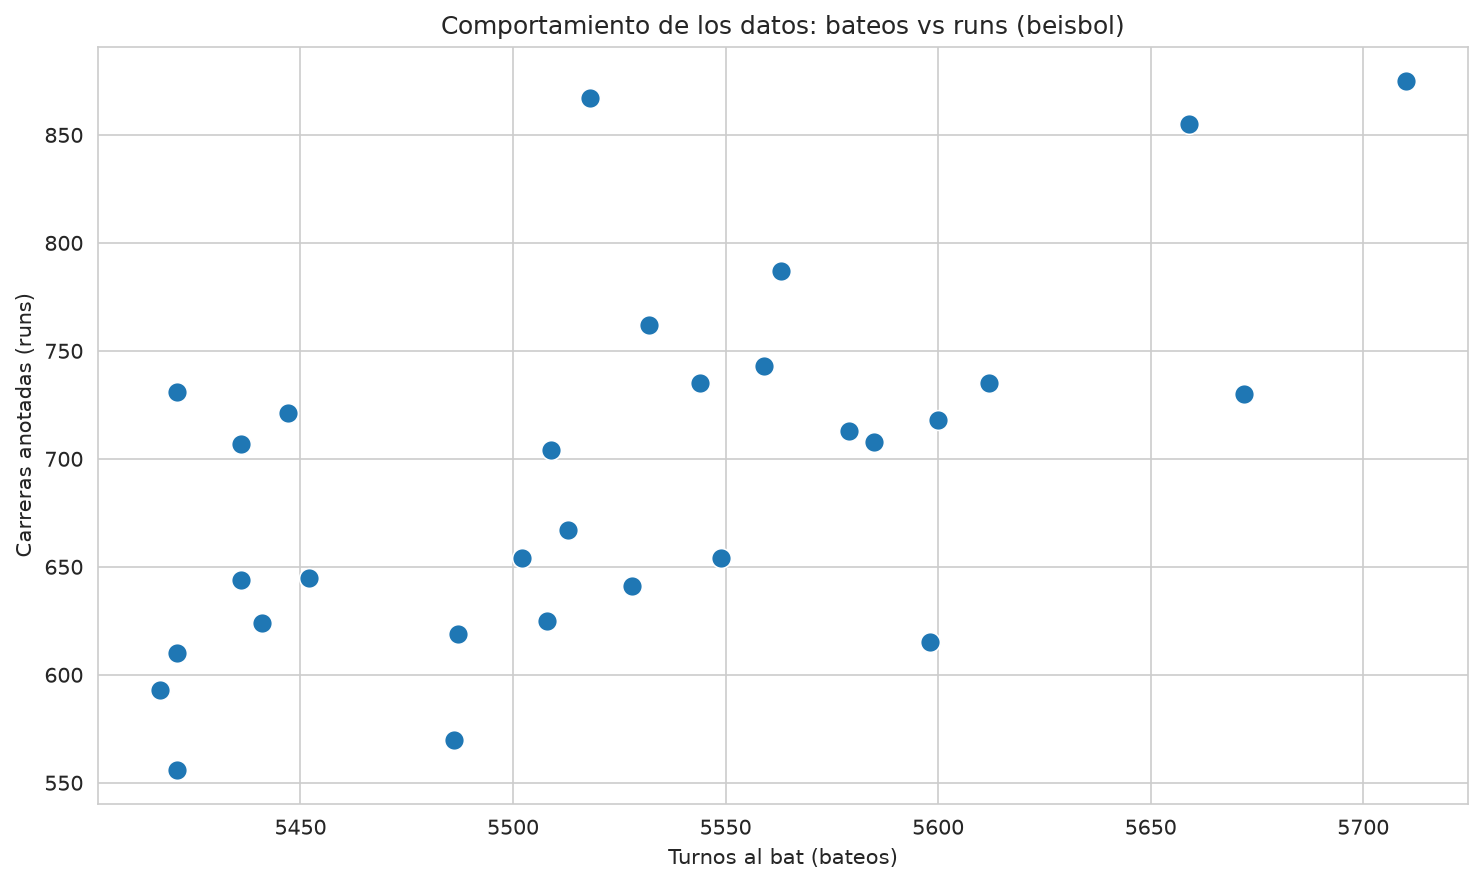
\includegraphics[width=0.82\linewidth]{img/scatter_beisbol_rf.png}
\caption{Dispersión del comportamiento de los datos (bateos vs runs).}
\end{figure}

\begin{figure}[H]
\centering
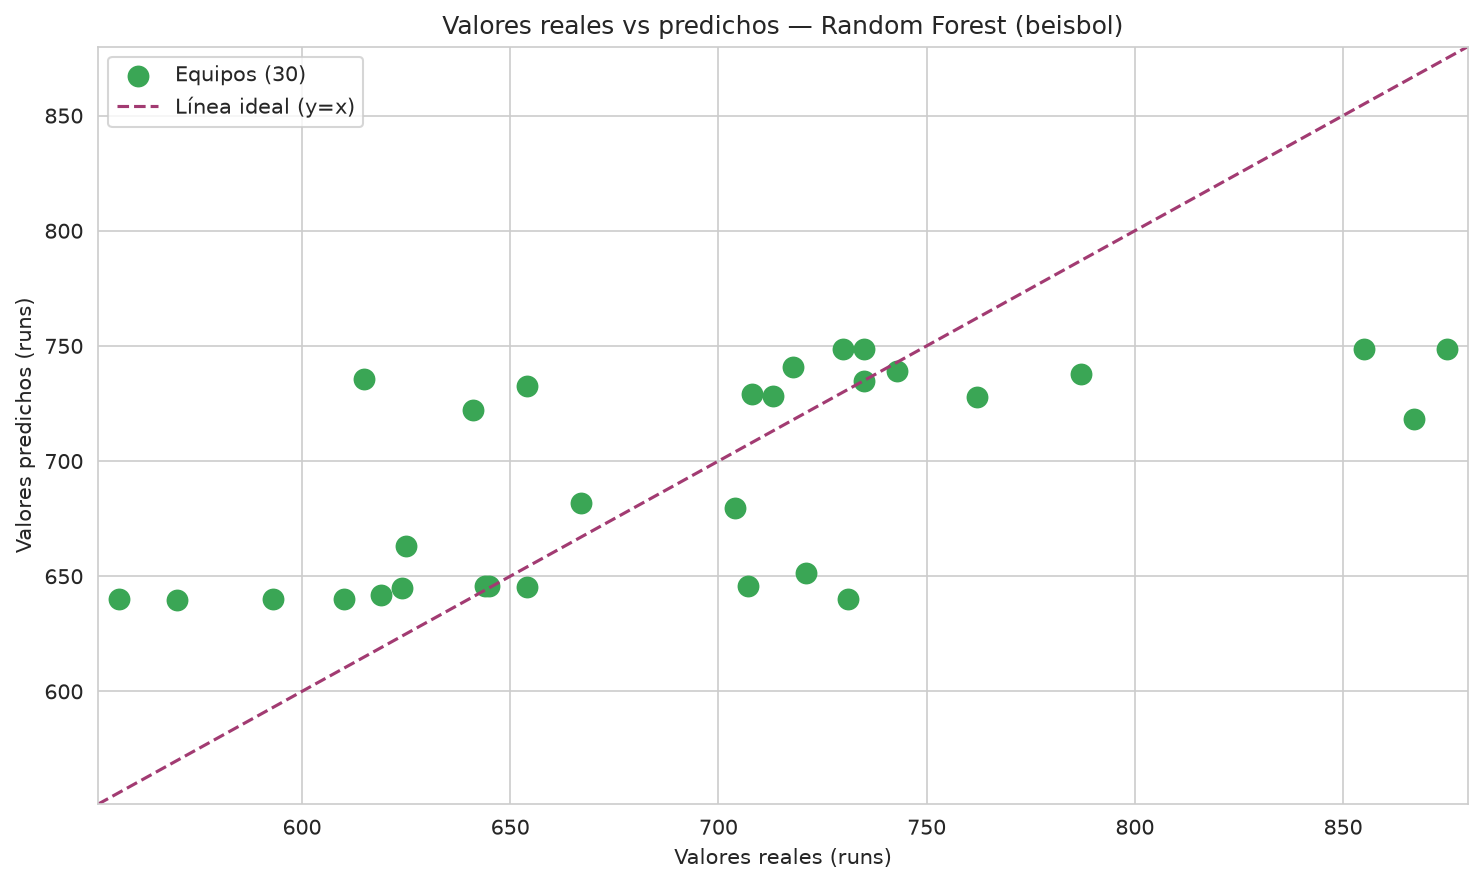
\includegraphics[width=0.82\linewidth]{img/reales_predichos_beisbol_rf.png}
\caption{Valores reales contra predichos para el Random Forest.}
\end{figure}

\textbf{Enlace al modelo:}
\begin{itemize}
\item Notebook: \url{https://github.com/rmMarioAlberto/evaluacion-u2-extraccion-conocimiento-bd/blob/main/notebooks/6_de_regresion_randomforest.ipynb}
\item Modelo: \url{https://github.com/rmMarioAlberto/evaluacion-u2-extraccion-conocimiento-bd/blob/main/modelos/beisbol_randomforest.pkl}
\end{itemize}

% ================= 7. AU =================
\section{Evaluación AU — Herramienta alternativa (Streamlit)}

\subsection{Justificación de la herramienta}
La evaluación AU solicita resolver los ejercicios de SA y DE con una
\textbf{herramienta alternativa a Jupyter Notebook}. Se eligió una
\textbf{aplicación web interactiva con Streamlit} (\texttt{app/streamlit\_app.py}),
que permite:
\begin{itemize}[itemsep=2pt]
\item ejecutar los seis modelos desde una interfaz gráfica,
\item visualizar métricas y gráficas de forma interactiva en pestañas,
\item demostrar el uso de una herramienta de despliegue de ciencia de datos distinta
      al entorno de notebooks.
\end{itemize}

\subsection{Diseño de la aplicación}
La aplicación carga los cuatro conjuntos de datos y organiza la solución en seis
pestañas (una por ejercicio): \textbf{SA Regresión (Lineal)}, \textbf{SA
Clasificación (k-NN)}, \textbf{NS Agrupación (K-Means)}, \textbf{NS Reducción
(PCA)}, \textbf{DE Clasificación (Random Forest)} y \textbf{DE Regresión (Random
Forest)}. Cada pestaña muestra la justificación, el preprocesamiento, las métricas
de evaluación y las gráficas correspondientes, reutilizando los hiperparámetros
óptimos encontrados en los notebooks.

\subsection{Reporte de evaluación y resultados en la app}
La aplicación reproduce las métricas de los notebooks:
\begin{table}[H]
\centering
\caption{Métricas mostradas en la app Streamlit}
\begin{tabular}{lcc}
\toprule
\textbf{Ejercicio} & \textbf{Métrica principal} & \textbf{Valor} \\
\midrule
SA Regresión (Lineal) & $R^2$ & 0.3729 \\
SA Clasificación (k-NN) & Accuracy & 0.9580 \\
NS Agrupación (K-Means) & Silueta & 0.4510 \\
NS Reducción (PCA) & Varianza (n=7) & 95.02\% \\
DE Clasificación (RF) & Accuracy & 0.9650 \\
DE Regresión (RF) & $R^2$ & 0.4060 \\
\bottomrule
\end{tabular}
\end{table}

\subsection{Capturas de la aplicación}
\begin{figure}[H]
\centering
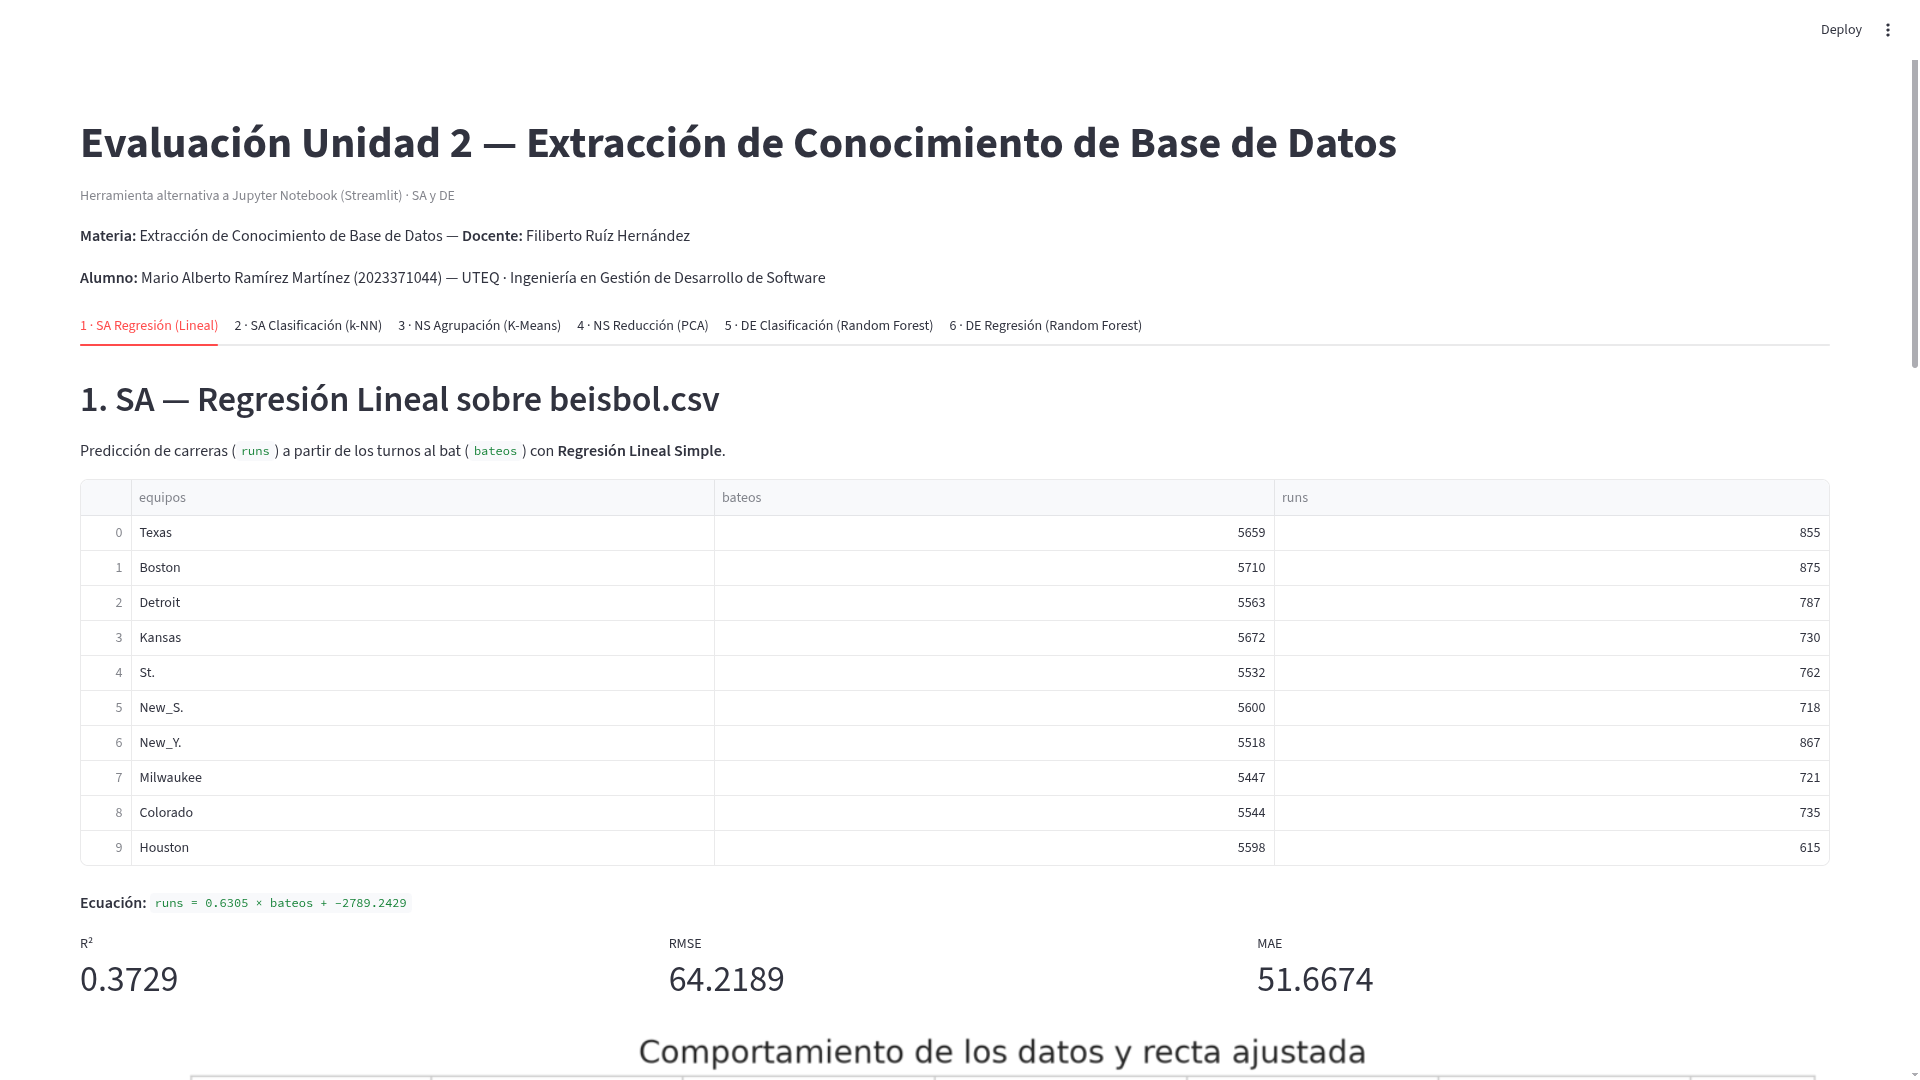
\includegraphics[width=0.9\linewidth]{img/au_tab1_regresion.png}
\caption{App Streamlit — pestaña 1: SA Regresión Lineal (beisbol).}
\end{figure}

\begin{figure}[H]
\centering
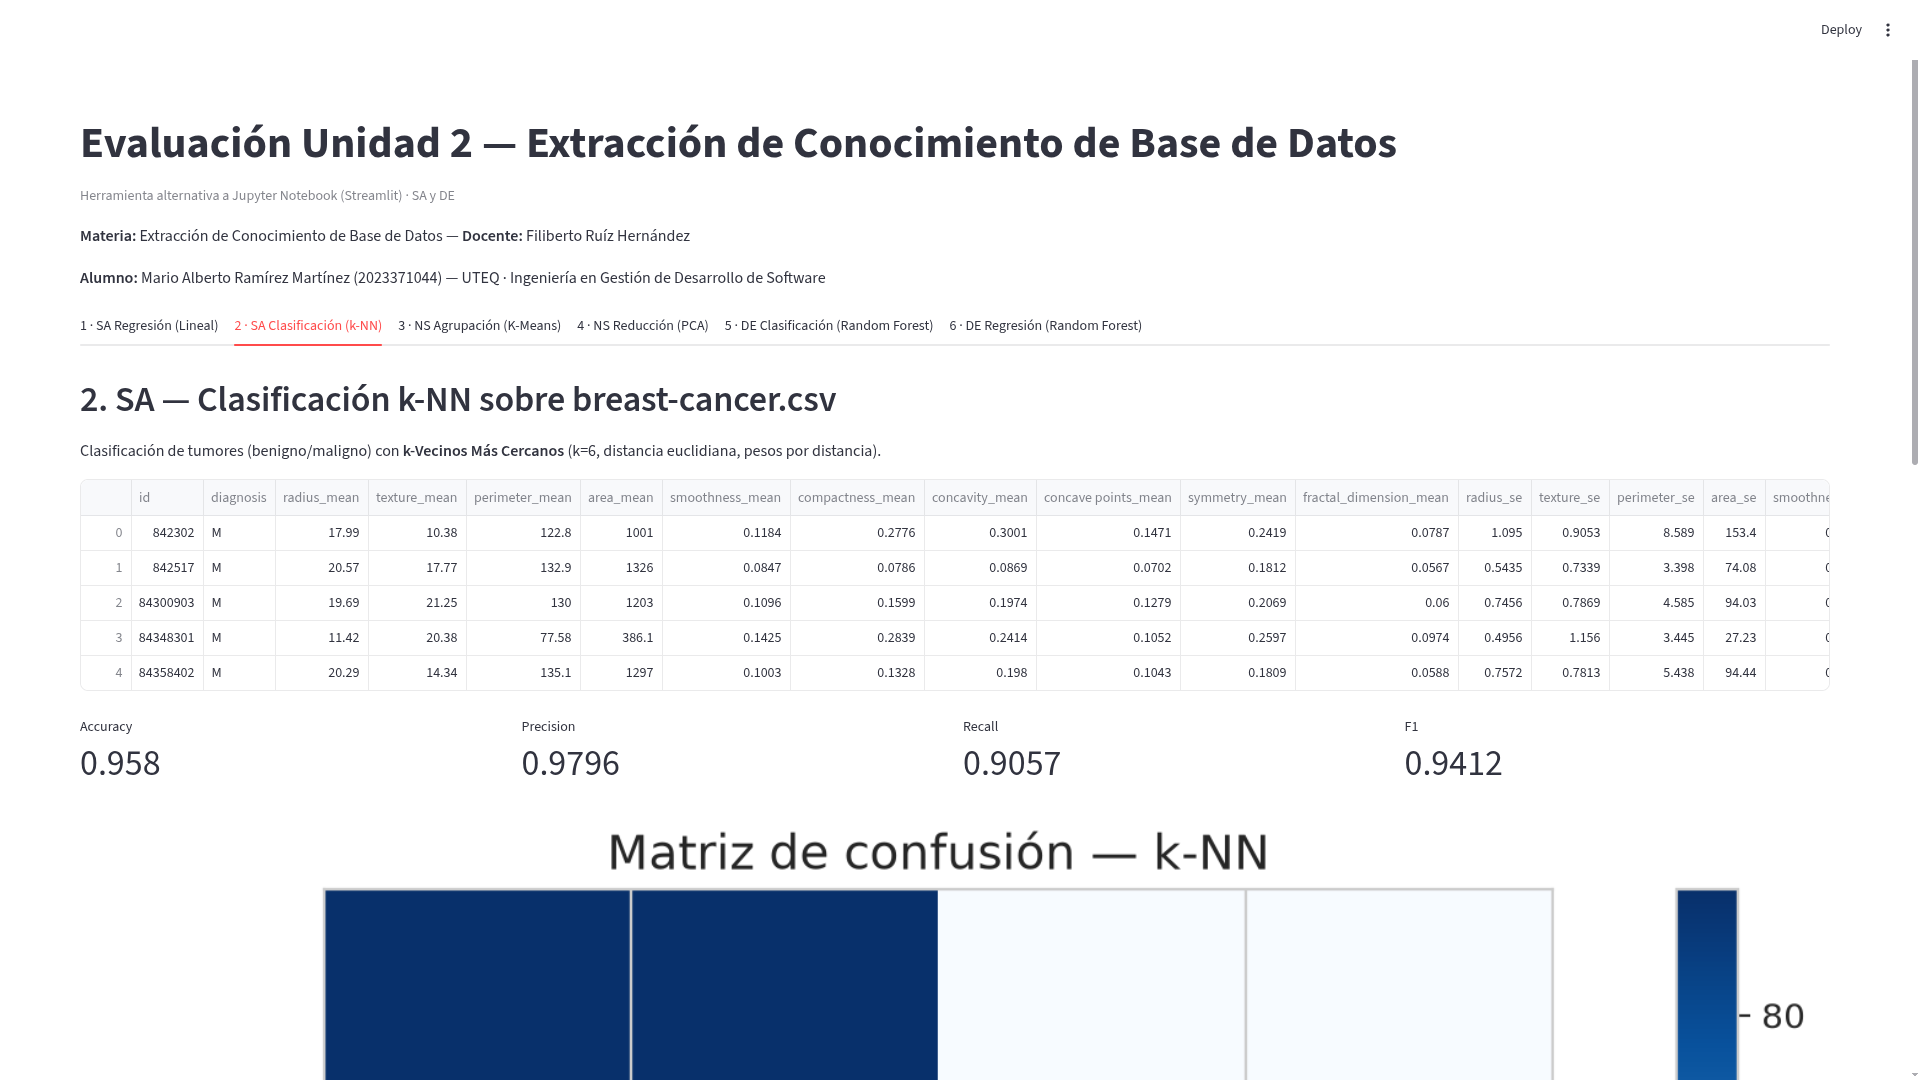
\includegraphics[width=0.9\linewidth]{img/au_tab2_knn.png}
\caption{App Streamlit — pestaña 2: SA Clasificación k-NN (breast-cancer).}
\end{figure}

\begin{figure}[H]
\centering
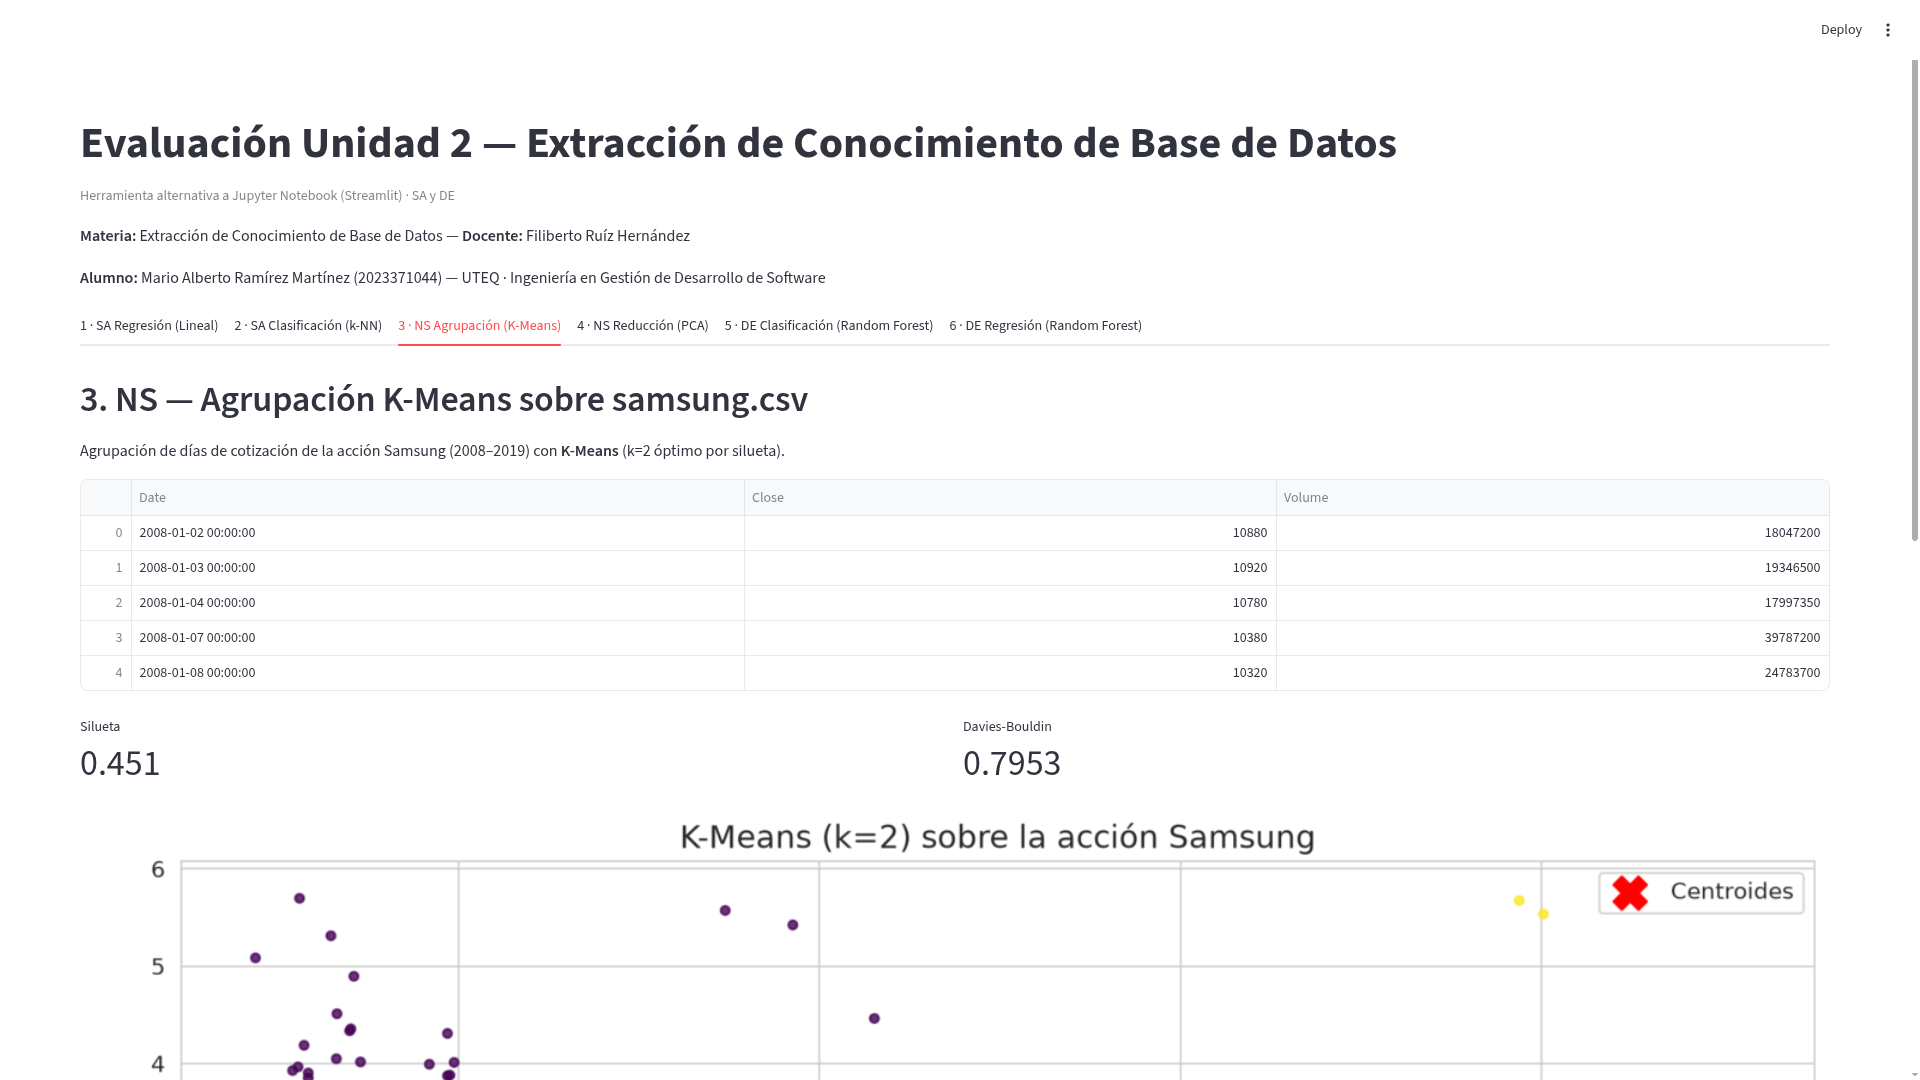
\includegraphics[width=0.9\linewidth]{img/au_tab3_kmeans.png}
\caption{App Streamlit — pestaña 3: NS Agrupación K-Means (samsung).}
\end{figure}

\begin{figure}[H]
\centering

\includegraphics[width=0.9\linewidth]{img/au_tab4_pca.png}
\caption{App Streamlit — pestaña 4: NS Reducción PCA (comprar\_alquilar).}
\end{figure}

\begin{figure}[H]
\centering
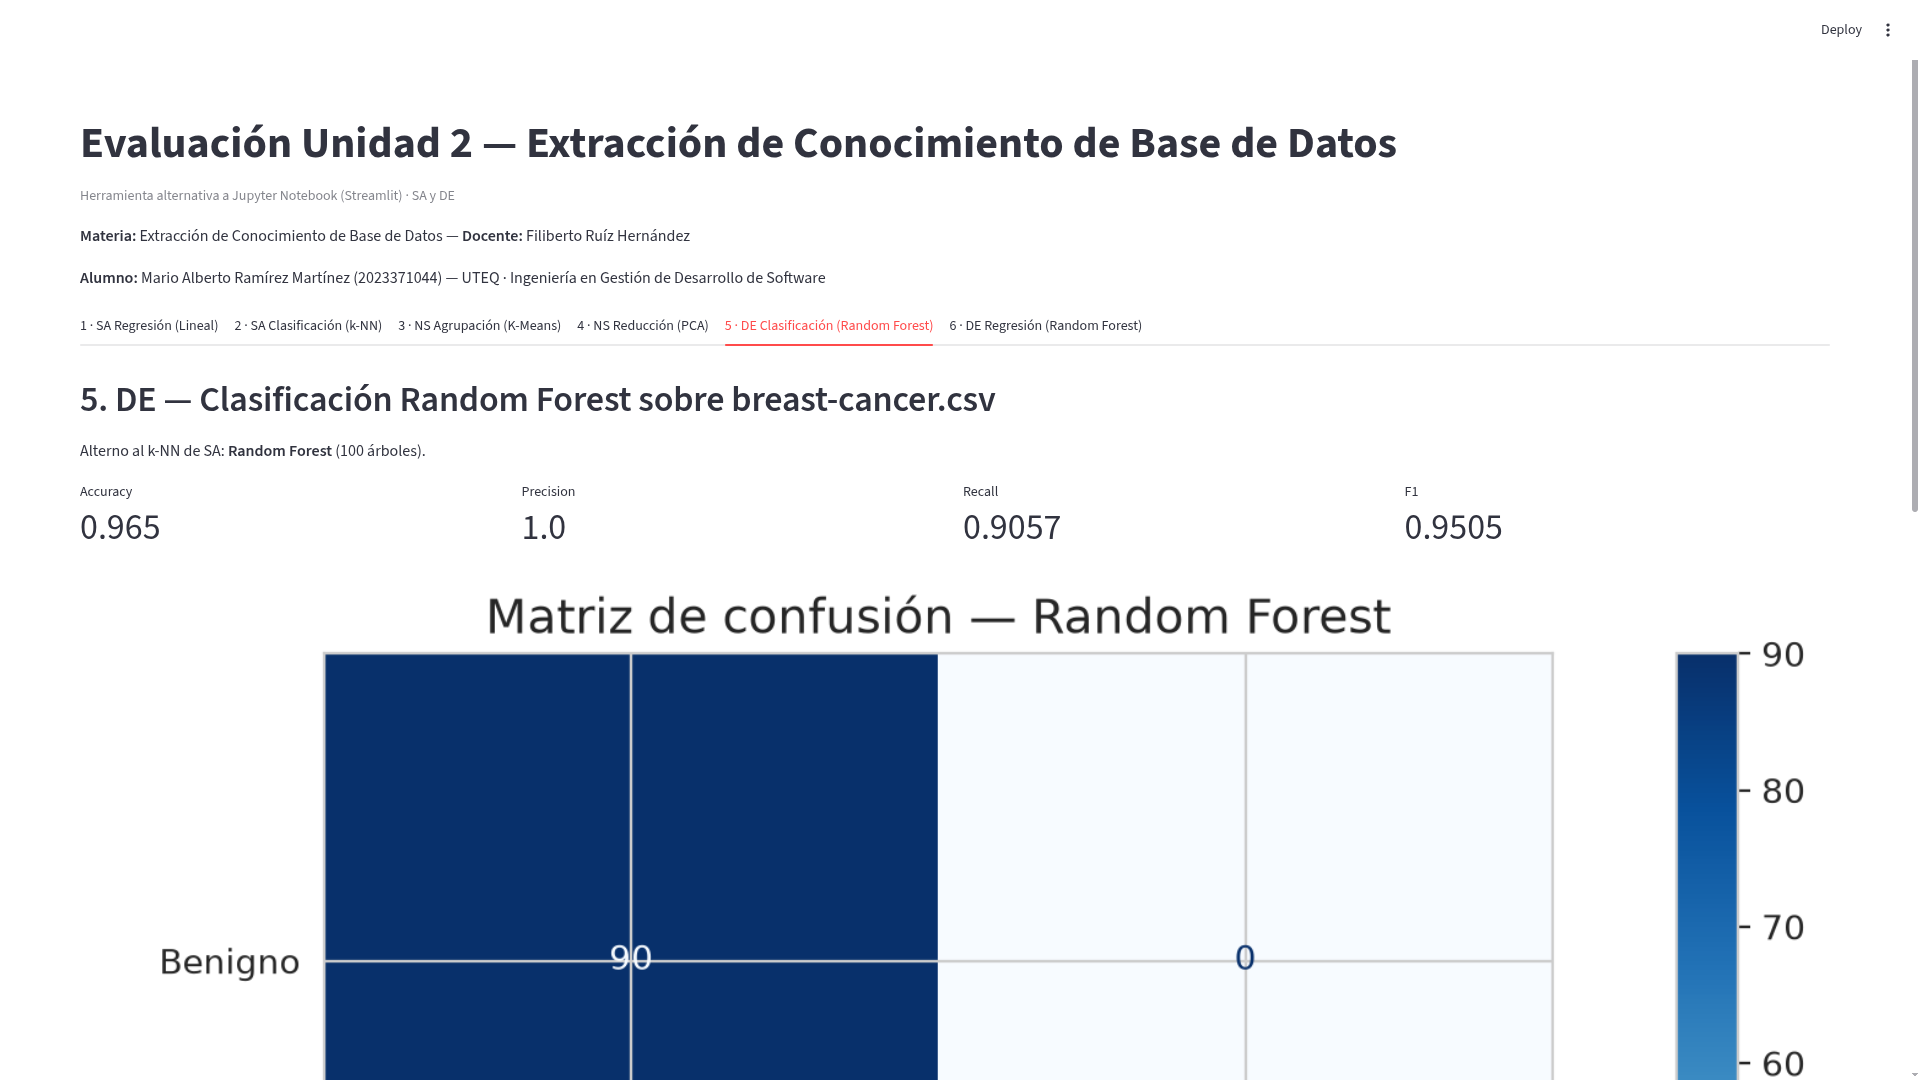
\includegraphics[width=0.9\linewidth]{img/au_tab5_rf_clf.png}
\caption{App Streamlit — pestaña 5: DE Clasificación Random Forest.}
\end{figure}

\begin{figure}[H]
\centering
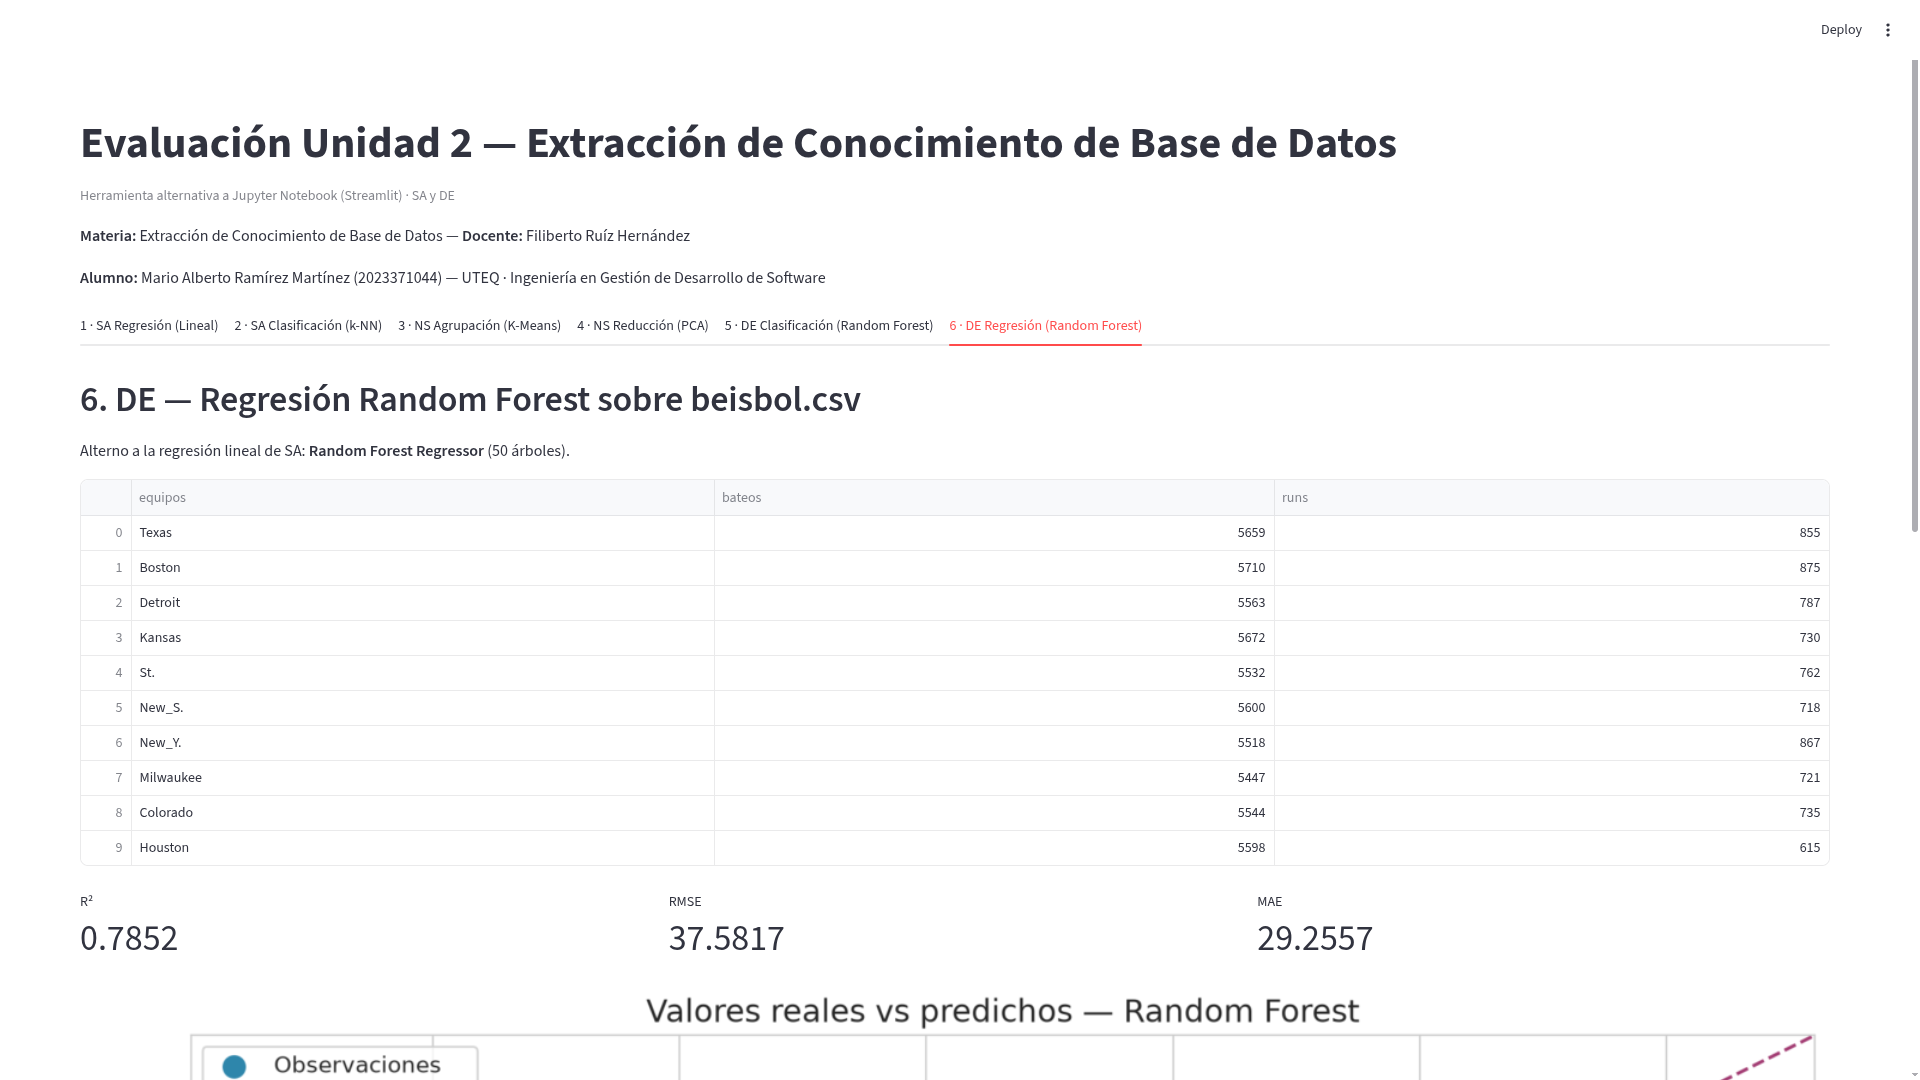
\includegraphics[width=0.9\linewidth]{img/au_tab6_rf_reg.png}
\caption{App Streamlit — pestaña 6: DE Regresión Random Forest.}
\end{figure}

\subsection{Enlace al repositorio}
Aplicación: \url{https://github.com/rmMarioAlberto/evaluacion-u2-extraccion-conocimiento-bd/blob/main/app/streamlit_app.py}

% ================= 8. CONCLUSIONES =================
\section{Conclusiones}
\begin{enumerate}[itemsep=3pt]
\item \textbf{Regresión (SA y DE).} Sobre \texttt{beisbol.csv} la regresión lineal
      explica el 37.3\% de la varianza de las carreras a partir de los turnos al
      bat; el Random Forest la mejora marginalmente (40.6\%). Con solo 30
      observaciones, la validación cruzada con RMSE resultó esencial para obtener
      estimaciones estables.
\item \textbf{Clasificación (SA y DE).} Sobre \texttt{breast-cancer.csv}, tanto k-NN
      (accuracy 0.958) como Random Forest (0.965) alcanzan un desempeño excelente;
      la optimización de hiperparámetros mejoró los resultados y las matrices de
      confusión muestran pocos falsos negativos (2 en k-NN, 5 en RF).
\item \textbf{Agrupación.} K-Means encontró dos regímenes de mercado en la serie de
      Samsung, validados por silueta (0.451) y Davies-Bouldin (0.795).
\item \textbf{Reducción de dimensionalidad.} El escalado es determinante: sin él
      PC1 concentra el 99\% de la varianza. Con \texttt{StandardScaler} se
      seleccionaron 7 componentes (95\% de varianza).
\item \textbf{Herramienta alternativa.} La aplicación Streamlit resuelve los seis
      ejercicios de forma interactiva, cumpliendo el requisito de AU con una
      herramienta distinta a Jupyter Notebook.
\end{enumerate}

% ================= 9. ANEXO =================
\section{Anexo — Repositorio del proyecto}
\begin{center}
\url{https://github.com/rmMarioAlberto/evaluacion-u2-extraccion-conocimiento-bd}
\end{center}

\begin{figure}[H]
\centering
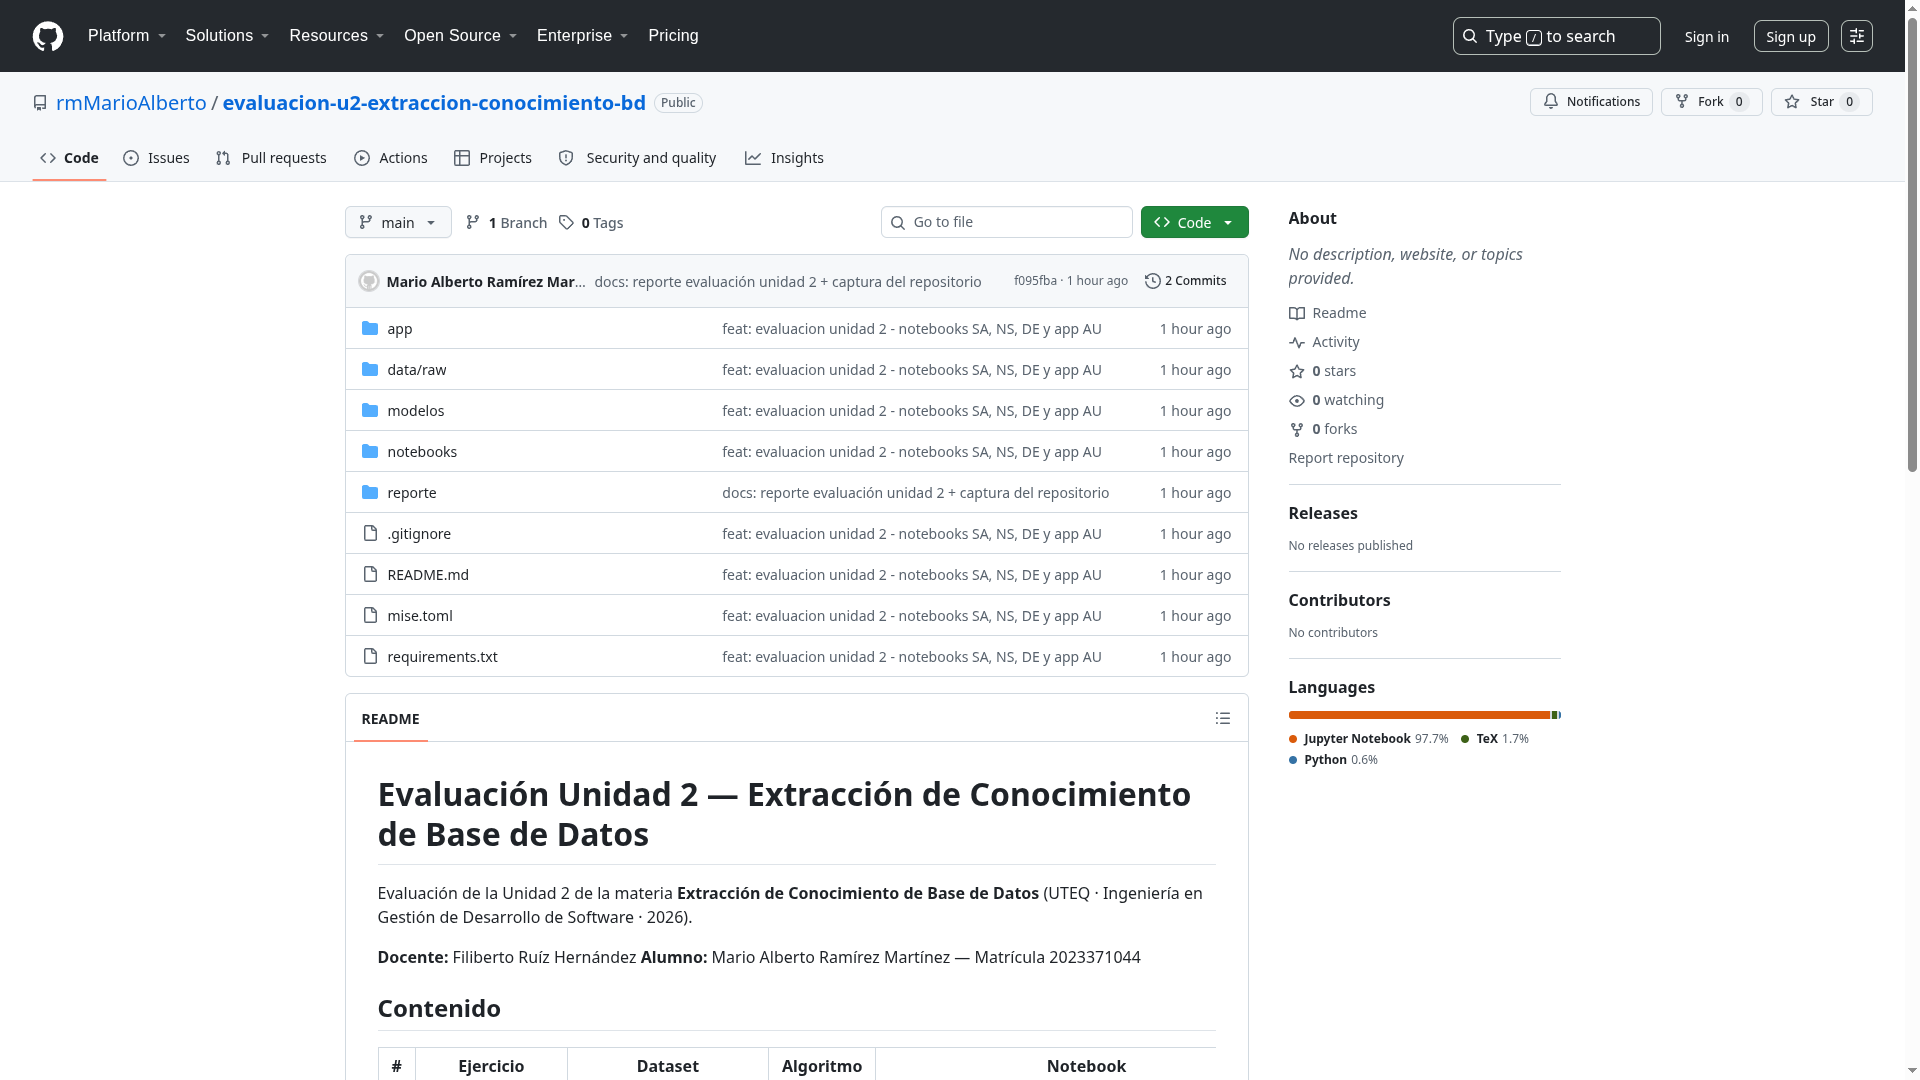
\includegraphics[width=\linewidth, height=0.6\textheight, keepaspectratio]{img/repo_github.png}
\caption{Captura del repositorio que contiene los notebooks, modelos, reporte y
aplicación de la evaluación.}
\end{figure}

\end{document}
